\chapter{\chatextprobReasoning}\label{cha:probReasoning}

After having investigated sparse decomposition schemes of probability distributions into tensor networks, we now exploit these schemes to derive efficient reasoning schemes. % Start of Focus Reasoning here
We first introduce by queries a generic scheme to retrieve information by contractions, and introduce the method of maximum likelihood estimation related to entropy optimization.
Then we focus on inference tasks in exponential families, which have been introduced as a generalization of graphical models in the previous chapter.


\sect{Queries}

The efficient retrieval of information stored in probability distributions has to exploit the available decomposition schemes.
To avoid the instantiation of a distribution based on its decomposition, we directly define deductive reasoning schemes by contractions, which can be executed using the available decomposition.

\subsect{Querying by functions}

We now formalize queries by retrieving expectations of functions given a distribution specified by probability tensors.
We exploit basis calculus in defining categorical variables $\headvariableof{\exfunction}$ to tensors $\exfunction$, which are enumerating the set $\imageof{\exfunction}$.
More details on this scheme are provided in \charef{cha:basisCalculus}, see \defref{def:functionRelationEncoding} therein.

\begin{definition}
    \label{def:queries}
    The marginal query of a probability distribution $\probat{\shortcatvariables}$ by a query statistic
    \begin{align*}
        \exfunction : \facstates \rightarrow \arbsetof{\exfunction}
    \end{align*}
    is the vector $\probat{\headvariableof{\exfunction}}$, where $\headvariableof{\exfunction}$ is an image enumerating variable (see \charef{cha:basisCalculus} for more details), defined as the contraction
    \begin{align*}
        \probat{\headvariableof{\exfunction}}
        = \contractionof{\probat{\shortcatvariables},\rencodingofat{\exfunction}{\headvariableof{\exfunction},\shortcatvariables}}{\headvariableof{\exfunction}} \, .
    \end{align*}
    If $\arbsetof{\exfunction}\subset\rr$, and the statistic $\exfunction$ is therefore a tensor, we further define the expectation query of $\probwith$ by $\exfunction$ as
    \begin{align*}
        \expectationof{\exfunction} = \sbcontraction{\exfunctionat{\shortcatvariables},\probwith} \, .
    \end{align*}
    Given another query statistic $\secexfunction: \facstates \rightarrow \arbsetof{\secexfunction}$, which image is enumerated by a variable $\headvariableof{\secexfunction}$, the conditional query of the probability distribution $\probat{\shortcatvariables}$ by the statistic $\exfunction$ conditioned on $\secexfunction$ is the matrix $\condprobof{\headvariableof{\exfunction}}{\headvariableof{\secexfunction}}\in\rr^{\cardof{\imageof{\exfunction}}}\otimes \rr^{\cardof{\imageof{\secexfunction}}}$ defined as the normation
    \begin{align*}
        \condprobof{\headvariableof{\exfunction}}{\headvariableof{\secexfunction}}
        = \normationofwrt{
            \probat{\shortcatvariables},\rencodingofat{\exfunction}{\headvariableof{\exfunction},\shortcatvariables},\rencodingofat{\secexfunction}{\headvariableof{\secexfunction},\shortcatvariables}
        }{
            \headvariableof{\exfunction}}{\headvariableof{\secexfunction}
        } \, .
    \end{align*}
\end{definition}

We notice, that marginal and conditional queries generalize the schemes of marginalization and conditioning on the distributed variables.
As such, marginal distributions are marginal queries with respect to a identity query statistic acting on the respective variables.
Conditional distributions can be similarly retrieved by two identity statistics, representing the incoming and outgoing variables.
%The query framework of \defref{def:queries} can be used beyond marginal and conditional quereis for the customized information retrieval.

%% Relation of queries and expectation queries
Expectation queries return the expectation of a real-valued feature $\exfunction : \facstates\rightarrow\rr$.
When understanding $\exfunction$ as a random variable given the probability measure $\probat{\shortcatvariables}$, the expectation query returns the expectation of that random variable.
Expectation queries are further contractions of marginal queries with the identity function restricted on the image of $\exfunction$, since
\begin{align*}
    \expectationof{\exfunction}
    = \contraction{\probat{\headvariableof{\exfunction}},\idrestrictedto{\imageof{\exfunction}}{\headvariableof{\exfunction}} } \, .
\end{align*}
This contraction equations follows from the more general \corref{cor:rhoToNormal}, which will be shown in \charef{cha:basisCalculus}.

%% Conditional Probabilities and conditional queries
%Conditional probabilities are queries, where the tensors $\exfunction$ and $\secexfunction$ are identity mappings in the respective variable state spaces.
%Conversely, we can understand the conditional query $\condprobof{\headvariableof{\exfunction}}{\headvariableof{\secexfunction}}$ as the conditional probability of a query statistic $\exfunction$ conditioned on $\secexfunction$, of the underlying Markov Network with cores $\{\probtensor, \rencodingof{\exfunction}, \rencodingof{\secexfunction} \}$ and variables $\catvariableof{\exfunction},\catvariableof{\secexfunction}$ besides the variables distributed by $\probtensor$.

%%% Expectations as event queries -> Consistency with $\probat{X=i}$?
%We further denote event queries by
%	\[  \expectationof{\exfunction=\exfunctionimageelement} = \sbcontraction{\probtensor,\rencodingof{\exfunction},\onehotmapof{\exfunctionimageelement}}\]
%where by $\onehotmapof{z}$ be denote the one hot encoding of the state $z$ with respect to some enumeration.
%Let us note that they are further contraction of the queries in \defref{def:queries} since by \theref{the:splittingContractions}
%\begin{align*}
%	 \expectationof{\exfunction=z}
%	& =  \sbcontraction{ \sbcontractionof{\probtensor,\rencodingof{\exfunction}}{\catvariableof{\exfunction}} ,\onehotmapof{z}}\\
%	& =  \sbcontraction{ \probat{\exfunction} ,\onehotmapof{z}} \, .
%\end{align*}

\subsect{Mode Queries}\label{sec:modeQueries}

A different kind of queries are mode queries, which we formalize by the searches of the indices to maximal coordinates in a tensor.

\begin{definition}
    Given a tensor $\hypercorewith$ the mode query is the problem
    \begin{align}
        \argmax_{\shortcatindicesin} \hypercoreat{\indexedshortcatvariables} \, .
    \end{align}
\end{definition}

%MAP relation - Needed?
%Mode queries are often called MAP queries.
%The name MAP is an abbreviation of maximum a-posteriori, since it searches for the most probable state in probability distributions.
%The term a-posteriori originates from a focus on conditional probabilities, which slices with respect to incoming variables represent the a-posteriori distribution given evidence on the incoming variables.
%We will in this work use this term for generic maximum coordinate searches.

% Convex optimization
We can pose mode queries as convex optimization problems.
To this end we recall, that the set of all probability distributions is a convex hull of the one-hot encoded states, that is
\begin{align*}
    \bmrealprobof{\ones}
    = \convhullof{\onehotmapofat{\shortcatindices}{\shortcatvariables} \, : \, \shortcatindicesin} \, .
\end{align*}
With this we have
\begin{align*}
    \max_{\shortcatindices} \hypercoreat{\indexedshortcatvariables}
    &= \max_{\shortcatindices} \contraction{\hypercoreat{\shortcatvariables},\onehotmapofat{\shortcatindices}{\shortcatvariables}} \\
    &= \max_{\meanparamat{\shortcatvariables}\in\bmrealprobof{\ones}} \contraction{\hypercoreat{\shortcatvariables},\meanparamat{\shortcatvariables}} \, .
\end{align*}
We note that the maximation over $\bmrealprobof{\ones}$ is a convex optimization problem and the maxima are taken at
\begin{align*}
    \argmax_{\meanparamat{\shortcatvariables}\in\bmrealprobof{\ones}} \contraction{\hypercoreat{\shortcatvariables},\meanparamat{\shortcatvariables}}
    = \convhullof{\onehotmapofat{\shortcatindices}{\shortcatvariables} \, : \, \shortcatindices\in\argmax_{\shortcatindices} \hypercoreat{\indexedshortcatvariables}} \, .
\end{align*}
We will further apply this generic trick to approach mode queries when studying inference problems for exponential families in the following sections.

% Restriction to subsets
Let us note, that we can also approach modified mode queries, where we restrict to $\arbset\subset\facstates$, namely
\begin{align*}
     \argmax_{\shortcatindices\in\arbset} \hypercoreat{\indexedshortcatvariables} \, .
\end{align*}
We can choose the base measure by the subset encoding (see \charef{cha:basisCalculus}) of $\arbset$, namely
\begin{align*}
    \basemeasurewith = \sum_{\shortcatindices\in\arbset} \onehotmapofat{\shortcatindices}{\shortcatvariables} \, ,
\end{align*}
and conclude that
\begin{align*}
    \argmax_{\meanparamat{\shortcatvariables}\in\bmrealprobof{\basemeasure}} \contraction{\hypercoreat{\shortcatvariables},\meanparamat{\shortcatvariables}}
    = \convhullof{\onehotmapofat{\shortcatindices}{\shortcatvariables} \, : \, \shortcatindices\in\argmax_{\shortcatindices\in\arbset} \hypercoreat{\indexedshortcatvariables}} \, .
\end{align*}



\subsect{Energy representations}

For exponential families (see \secref{sec:exponentialFamilies}) we have observed, that often energy tensors have feasible tensor network representations, whereas the corresponding probability distributions can get infeasible.
We therefore investigate here schemes to answer queries based on the energy tensor instead of the distribution.
%Let us now interpret a probability tensor at hand as a member of an exponential family (see \secref{sec:exponentialFamilies}), which is always possible when taking the naive exponential family.

\begin{theorem}
    \label{the:energyContractionQueries} % This is a statement about "full" queries.
    Let $\energytensorat{\shortcatvariables}$ be an energy tensor and $\probwith=\normationof{\expof{\energytensorat{\shortcatvariables}}}{\shortcatvariables}$ the corresponding distribution.
%	For any probability distribution $\probtensor$ with $\probtensor= \normationof{\expof{\energytensorat{\shortcatvariables}}}{\shortcatvariables}$,
    For disjoint subsets $\nodesa,\nodesb \subset [\catorder]$ with $\nodesa\cup\nodesb=[\catorder]$ and any $\catindexof{\nodesb}$ we have
    \begin{align*}
        \condprobof{\catvariableof{\nodesa}}{\indexedcatvariableof{\nodesb}}
        = \normationof{
            \expof{\energytensorat{\catvariableof{\nodesa},\indexedcatvariableof{\nodesb}}}
        }{\catvariableof{\nodesa}} \, .
    \end{align*}
\end{theorem}
\begin{proof}
    To show the theorem, we use a generic simplification property of coordinatewise transforms, which we will show as \lemref{lem:coordinatewisetrafoSliceReduction} in \charef{cha:coordinateCalculus} and get
    \begin{align*}
        \contractionof{\expof{\energytensorat{\catvariableof{\nodesa},\catvariableof{\nodesb}}}}{\catvariableof{\nodesa},\indexedcatvariableof{\nodesb}}
        = \contractionof{\expof{\energytensorat{\catvariableof{\nodesa},\indexedcatvariableof{\nodesb}}}}{\catvariableof{\nodesa}}
    \end{align*}
    Based on this we get
    \begin{align*}
        \condprobof{\catvariableof{\nodesa}}{\indexedcatvariableof{\nodesb}}
        = \normationofwrt{\expof{\energytensorat{\catvariableof{\nodesa},\catvariableof{\nodesb}}}}{\catvariableof{\nodesa}}{\indexedcatvariableof{\nodesb}} \\
        = \frac{\contractionof{\expof{\energytensorat{\catvariableof{\nodesa},\catvariableof{\nodesb}}}}{\catvariableof{\nodesa},\indexedcatvariableof{\nodesb}}}{
            \contractionof{\expof{\energytensorat{\catvariableof{\nodesa},\catvariableof{\nodesb}}}}{\indexedcatvariableof{\nodesb}}
        } \\
        = \frac{\contractionof{\expof{\energytensorat{\catvariableof{\nodesa},\indexedcatvariableof{\nodesb}}}}{\catvariableof{\nodesa}}}{
            \contraction{\expof{\energytensorat{\catvariableof{\nodesa},\indexedcatvariableof{\nodesb}}}}
        } \\
        = \normationof{
            \expof{\energytensorat{\catvariableof{\nodesa},\indexedcatvariableof{\nodesb}}}
        }{\catvariableof{\nodesa}} \, .
    \end{align*}
\end{proof}

% Situation of marginalized variables
Importantly, \theref{the:energyContractionQueries} does not generalize to situations, where $\nodesa\cup\nodesb\neq[\catorder]$, since summation over the indices of the variables $[\catorder]/\nodesa\cup\nodesb$ and contraction do not commute.
In this more generic situation, we would need to sum over exponentiated coordinates, that is
\begin{align*}
    \condprobof{\catvariableof{\nodesa}}{\indexedcatvariableof{\nodesb}}
    = \normationof{
        \sum_{\catindexofin{[\catorder]/\nodesa\cup\nodesb}}
        \expof{\energytensorat{\catvariableof{\nodesa},\indexedcatvariableof{\nodesb},\indexedcatvariableof{[\catorder]/\nodesa\cup\nodesb}}}
    }{\catvariableof{\nodesa}} \, .
\end{align*}


% Mode queries
Mode queries on probability distributions in an energy representation can always be reduces to mode queries on the energy tensor.
This is due to the monotonicity of the exponential function, which implies
\begin{align*}
    \argmax_{\shortcatindicesin} \probat{\indexedshortcatvariables}
    &=\argmax_{\shortcatindicesin} \normationof{\expof{\energytensorat{\shortcatvariables}}}{\indexedshortcatvariables} \\
    &=\argmax_{\shortcatindicesin} \expof{\energytensorat{\indexedshortcatvariables}} \\
    &=\argmax_{\shortcatindicesin} \energytensorat{\indexedshortcatvariables} \, .
\end{align*}
Since we are only interested in identifying the index of the maximum coordinate, and not its value, we have further dropped the normalization term by partition functions.
When one instead need to get the value of the maximal, the partition function cannot be ignored.

\sect{Sampling}

Let us here investigate how to draw samples from a prbability distribution, based on queries on it.
Naive methods, such as drawing a random number in $[0,1]$, adding iteratively the coordinates and stopping when the sum exceeds the random variables, are infeasible when having large tensor orders causing exponential increases of the coordinate number.
We recall, that the number of coordinates of $\probwith$ is $\prod_{\catenumeratorin}\catdimof{\catenumerator}$, which increases exponentially in the number $\catorder$ of the variables.
Efficient methods instead have to exploit tensor network decompositions of the decompositions.

\subsect{Exact Methods}

The first insight to derive efficient sampling algorithms is to sample a single variable in each step.
Forward sampling (see \algoref{alg:ForwardSampling}) exploits to this end the generic chain decomposition (see \theref{the:chainRule}) of a probability distribution, namely
\begin{align*}
    \probwith = \contractionof{\{\margprobat{\catvariableof{0}}\} \cup
    \left\{\condprobof{\catvariableof{\catenumerator}}{\catvariableof{0},\ldots,\catvariableof{\catenumerator-1}}\,:\,\catenumeratorin, \, \catenumerator\geq 1\right\}
    }{\shortcatvariables} \, ,
\end{align*}
It then samples iteratively a state $\catindexof{\catenumerator}$ for the variable $\catvariableof{\catenumerator}$ conditioned on the previously sampled states, that is from the conditonal distribution
\begin{align*}
    \condprobof{\catvariableof{\catenumerator}}{\indexedcatvariableof{[\catenumerator]}} \, .
\end{align*}
The generic chain decomposition thereby ensures that probability of getting a state $\shortcatindices$ by this procedure coincides with $\probat{\indexedshortcatvariables}$.

\begin{algorithm}[hbt!]
    \caption{Forward Sampling}\label{alg:ForwardSampling}
    \begin{algorithmic}
        \For{$\catenumeratorin$}
            \State Draw $\catindexof{\catenumerator}\in[\catdimof{\catenumerator}]$ from the conditional distribution
            \begin{align*}
                \condprobof{\catvariableof{\catenumerator}}{\indexedcatvariableof{[\catenumerator]}}
            \end{align*}
        \EndFor
    \end{algorithmic}
\end{algorithm}

% Bayesian networks
Forward Sampling is especially efficient, when sampling from a Bayesian Network respecting the topological order of its nodes.
More technically, when the parents $\parentsof{\catenumerator}$ of a node $\catenumerator$ are contained in the preceding variables $[\catenumerator]$, we apply the conditional independence assumption (more precisely \theref{the:conditionDropping} in combination with \theref{the:condIndBN}) to get
\begin{align*}
    \condprobof{\catvariableof{\catenumerator}}{\indexedcatvariableof{[\catenumerator]}}
    = \condprobof{\catvariableof{\catenumerator}}{\indexedcatvariableof{\parentsof{\catenumerator}}} \, .
\end{align*}
Since this conditional probability coincides with a local tensor in the Bayesian Network, we can avoid to contract the network for preparing the conditional distribution.
Different to more general Markov Networks, forward sampling from Bayesian Network can therefore be done efficiently by reduction to conditional queries answerable using local tensors.
We note that it is important to sample in the topological order induced by the underlying directed hypergraph, since the computation of generic conditional distributions is also for Bayesian Networks $\mathsf{NP}$-hard (see Chapter~13 in \cite{koller_probabilistic_2009}).
Sampling along the topological variable order requires only tractable to answer conditional queries on the Bayesian Network.

%% Comment on rejection Sampling 
%When sampling from conditional probability distributions, one can sample from the conditioned distribution instead.
%However, the conditioning changes the structure of the distribution, and conditioned Bayesian Networks are not Bayesian Networks on the same graph.
%One ways around is rejection sampling, where one samples from the unconditioned distribution and rejects samples not satisfying the event conditioned on.
%When the event conditioned on is of small probability, methods like rejection sampling will come with large runtimes.

\subsect{Gibbs Sampling}

While we have seen that forward sampling can be performed efficiently on Bayesian Networks, Gibbs sampling can be also performed efficiently for Markov Networks.
Gibbs sampling \algoref{alg:Gibbs} overcomes the intractability problems of sampling steps during forward sampling at the expense of repetitions of the sampling step.
%The tractability of each sampling step is traded off against the number of repetitions to produce a sample.
When performing finite repetitions, Gibbs sampling in general samples from an approximate distribution to the one desired.
It can be shown, that these approximate distribution tend to one desired in the asymptotic limit of infinite repetitions of the sampling step (see Chapter~12 in \cite{koller_probabilistic_2009}).

\begin{algorithm}[hbt!]
    \caption{Gibbs Sampling}\label{alg:Gibbs}
    \begin{algorithmic}
        \For{$\catenumeratorin$}
            \State Draw $\catindexof{\catenumerator}$ from an initialization distribution. % In implementation: Initialize with ones and draw -> Avoids zero probability state
        \EndFor
        \While{Stopping criterion is not met}
            \For{$\catenumeratorin$}
                \State Draw $\catindexof{\catenumerator}$ from the conditional distribution
                \begin{align*}
                    \condprobof{\catvariableof{\catenumerator}}{\indexedcatvariableof{[\catorder]/\{\catenumerator\}}}
                \end{align*}
            \EndFor
        \EndWhile
    \end{algorithmic}
\end{algorithm}

% Efficiency on Markov Networks
The central problem of forward sampling on Markov Networks has been the need for global contractions to answer the required conditional queries, which originates from large numbers of variables to be marginalized out.
When avoiding the marginalization of variables, and conditioning on them instead, global contractions can be avoided.
To be more precise, for any tensor network $\extnet$ on $\graph=([\catorder],\edges)$ and any $\catenumeratorin$ we have
\begin{align*}
    \contractionof{\extnet}{\catvariableof{\catenumerator},\catvariableof{[\catorder]/\{\catenumerator\}}}
    = \contractionof{\{\hypercoreat{\edge}{\catvariableof{\catenumerator},\indexedcatvariableof{\edge/\{\catenumerator\}}} \, : \, \edge\in\edges, \, \catenumerator\in\edge\}}{\catvariableof{\catenumerator}}
    \cdot \prod_{\edge\in\edges, \, \catenumerator\notin\edge} \hypercoreat{\edge}{\indexedcatvariableof{\edge}} \, .
\end{align*}
As a consequence, we get for the Markov Network $\probtensor=\probof{\graph}$ to $\extnet$, that
\begin{align*}
    \condprobof{\catvariableof{\catenumerator}}{\indexedcatvariableof{[\catorder]/\{\catenumerator\}}}
    &= \normationof{\extnet}{\catvariableof{\catenumerator},\catvariableof{[\catorder]/\{\catenumerator\}}} \\
    &= \normationof{\{\hypercoreat{\edge}{\catvariableof{\catenumerator},\indexedcatvariableof{\edge/\{\catenumerator\}}} \, : \, \edge\in\edges, \, \catenumerator\in\edge\}}{\catvariableof{\catenumerator}} \, .
\end{align*}
The conditional queries on a Markov Network asked in Gibbs Sampling can therefore be answered by contractions only of those tensors containing the variable $\catvariableof{\catenumerator}$.
To find further locally answerable conditional queries, we need to condition only on the neighbored variables, refered to as Markov blanket, such that the other variables are conditionally independent.
This follows from the characterization of the conditional independences eminent in Markov Networks, which has been shown in \theref{the:condIndMN}, and can be used to design further tractable sampling schemes for Markov Networks.

% Energy
We can further answer these conditional queries efficiently, when we perform Gibbs sampling on a probability distribution in an energy representation, that is $\probwith=\normationof{\expof{\energytensorat{\shortcatvariables}}}{\shortcatvariables}$.
Using \theref{the:energyContractionQueries}, we have
\begin{align*}
    \condprobof{\catvariableof{\catenumerator}}{\indexedcatvariableof{[\catorder]/\{\catenumerator\}}}
    = \normationof{\expof{\energytensorat{\catvariableof{\catenumerator},\indexedcatvariableof{[\catorder]/\{\catenumerator\}}}}
    }{\catvariableof{\nodesa}}
\end{align*}
We note, that the main property of the conditional query exploited here, is that all variables but the one sampled appear as a condition and none is marginalized out.
In the scheme of forward sampling, where most of the variables are marginalized out in many queries, we cannot apply this trick and would have to perform sums over exponentiated coordinates to the variables marginalized out.


\subsect{Simulated Annealing}\label{sec:simulatedAnnealing}

Simulated annealing is an adapted sampling scheme that targets mode queries rather than generating representative samples from a distribution.
It employs an annealing process that gradually transforms the probability distribution by increasingly favoring high-likelihood configurations, thereby improving the chances of sampling a solution to a mode query.
To be more precise, let there be a distribution in energy representation, that is $\probwith=\normationof{\expof{\energytensorat{\shortcatvariables}}}{\shortcatvariables}$.
Whe introduce a parameter $\invtemp\in\rr$, which we understand as the inverse temperature, and anneal the distribution through scaling its energy by this parameter.
%\begin{align*}
%    \energytensorofat{\invtemp}{\shortcatvariables} = \invtemp \cdot \energytensorat{\shortcatvariables} \, .
%\end{align*}
In the limit of $\invtemp\rightarrow\infty$, for each state $\shortcatindicesin$ the annealed distribution behaves as
\begin{align*}
    \normationof{\expof{\invtemp\cdot\energytensorofat{\shortcatvariables}}}{\indexedshortcatvariables} \rightarrow
    \normationof{\ones_{\argmax_{\shortcatindicesin}\energytensorat{\indexedshortcatvariables}}}{\indexedshortcatvariables} \, .
\end{align*}
In this limit, the annealed distribution tends to the uniform distribution of the maximal coordinates, that is the uniform distribution of the set
\begin{align*}
    \argmax_{\shortcatindicesin}\energytensorat{\indexedshortcatvariables} = \argmax_{\shortcatindicesin}\probat{\indexedshortcatvariables} \, .
\end{align*}

To integrate annealing into Gibbs sampling, one chooses a parameter $\invtemp$ for each repetition of a sampling step and sample from the conditioned annealed distribution $\normationof{\expof{\invtemp\cdot\energytensorat{\shortcatvariables}}}{\shortcatvariables}$.
Through increasing $\invtemp$ during the algorithm, the samples are drawn towards states with larger coordinates in $\probat{\shortcatvariables}$.
However, when $\invtemp$ is large, the sampling procedure can get stuck in local maxima, whereas small $\invtemp$ are in favor of overcoming such.
The inverse temperature is thus understood as a tradeoff parameter between the exploration of new regions of the state space and increasing the coordinate of the sample by local coordinate optimization.
It is therefore typically chosen low in the beginning of the sampling algorithm and then sequentially increased to find maximal coordinates.
Due to this typical increasement of the inverse temperature strategy, the algorithm is refered to as simulated annealing.


\sect{Maximum Likelihood Estimation} % Stuff from Parameter Estimation - Problem that Part I is called inference?

So far we have been concerned with deductive reasoning task, that is retrieve information from a given distribution or drawing a sample.
We now turn to inductive reasoning tasks, where a probability distribution is estimated given data.
To present the generic framework of maximum likehihood estimation in the tensor network contraction formalism, we introduce the likelihood loss exploiting the structure of empirical distribution, and then provide interpretations in terms of entropies.

\subsect{Likelihood Loss}

Following the notation in \secref{sec:empDistribution}, datasets $\dataset$ are collections of observed samples
\begin{align*}
    \datamapat{\datindex} = (\catindicesof{\datindex}) \in \facstates
\end{align*}
of a factored system.
The likelihood of a probability distribution $\probwith$ to produce an observed sample is then
\begin{align*}
    \probat{\shortcatvariables = \datamapat{\datindex}} \, .
\end{align*}
We further introduce the likelihood of $\probwith$ with respect to a dataset as
\begin{align*}
    \probat{\dataset} := \prod_{\datindexin} \probat{\shortcatvariables = \datamapat{\datindex}} \, .
\end{align*}
The likelihood draws on the assumption, that each datapoint in the dataset has been drawn independently from the same distribution.
When this generating distribution coincides with $\probwith$, then the probability of generating a dataset by this scheme is the likelihood.
In inductive reasoning, the true distribution $\probwith$ is unknown and needs to be approximatively estimated based on data and a learning hypothesis.
We will therefore compute and compare the likelihood of distributions, which in general do not coincide with the distribution generating the data.
It is thus important to not understand the likelihood as a probability, which is only true for the generating distribution, as pointed out in Chapter~2 in \cite{mackay_information_2003}.

% Logarithm
Let us now transform the likelihood to find an representation involving the empirical distribution (see \defref{def:dataMap}), for which efficient tensor network decompositions have been derived in \theref{the:empCPRep}.
Applying a scaled logarithm we get
\begin{align*}
    \frac{1}{\datanum} \cdot \lnof{\probat{\dataset}}
    &= \frac{1}{\datanum} \cdot \lnof{\prod_{\datindexin} \probat{\shortcatvariables = \datamapat{\datindex}}} \\
    &= \dataaverage \lnof{\probat{\shortcatvariables = \datamapat{\datindex}}} \\
    &= \contractionof{\lnof{\probwith},\empdistributionwith} \, .
\end{align*}
Let us notice, that this transform of the likelihood is monotoneous and therefore does not influence the position of the maximum, when optimizing the likelihood.
Motivated by this property, we use the transformed form to define the loss-likelihood loss and maximum likelihood estimation.
%This is especially useful, when investigating the convergence of the objective for $\datanum\rightarrow\infty$ (see \charef{cha:concentration}).

\begin{definition}
    \label{def:loss}
    The log-likelihood loss of a distribution $\probtensor$ given a dataset $\dataset$ is the functional
    \begin{align*}
        \lossof{\probtensor}
        = -\contractionof{\lnof{\probwith},\empdistributionwith} \, .
    \end{align*}
    Having a hypothesis $\Gamma\subset\bmrealprobof{\ones}$, that is a set of probability distributions, the maximum likelihood estimation is the problem
    \begin{align}
        \tag{$\probtagtypeinst{\loss}{\Gamma,\empdistribution}$}\label{prob:parameterMaxLikelihood}
        \argmin_{\probtensor\in\Gamma} \lossof{\probtensor} \, .
    \end{align}
\end{definition}


\subsect{Entropic Interpretation}

The Shannon entropy, which has been introduced in the seminal paper \cite{shannon_mathematical_1948}, is a foundational concept in various research fields beyond statistical learning, such as information theory or statistical physics.
While a detailed discussion is out of the scope of this work, we here only provide computation schemes of the entropy based on contractions of distributions.

\begin{definition}[Shannon entropy]
    The Shannon entropy of a distribution $\probwith$ is the quantity
    \begin{align*}
        \sentropyof{\probtensor}
        =  \sum_{\shortcatindicesin} \probat{\indexedshortcatvariables} \cdot \left(-\lnof{\probat{\indexedshortcatvariables}}\right)
        = \sbcontraction{\probtensor,-\lnof{\probtensor}} \, .
    \end{align*}
    We represent the Shannon entropy by the tensor network diagram
    \begin{center}
        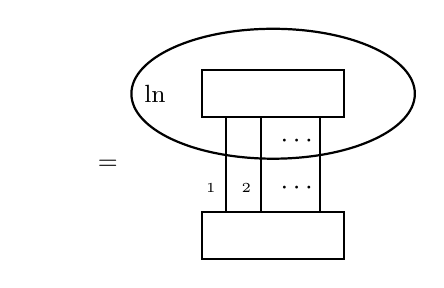
\begin{tikzpicture}[scale=0.3,thick] % , baseline = -3.5pt

\node[anchor=center] (text) at (-8,-5) {\small $\sentropyof{\probtensor}$};

\node[anchor=center] (text) at (-5,-5) {\small ${=}$};

\node[anchor=center] (text) at (-3,-2) {\small $\mathrm{ln}$};
\draw (2,-2) ellipse (6 and 2.75);

\draw (-1,-1) rectangle (5,-3);
\node[anchor=center] (text) at (2,-2) {\small $\probtensor$};
\draw (-1,-7) rectangle (5,-9);
\node[anchor=center] (text) at (2,-8) {\small $\probtensor$};
\draw (0,-5)--(0,-3); 
\draw (0,-5)--(0,-7) node[midway,left] {\tiny $\atomlegindexof{1}$}; 
\draw (1.5,-5)--(1.5,-3); 
\draw (1.5,-5)--(1.5,-7) node[midway,left] {\tiny $\atomlegindexof{2}$}; 
\node[anchor=center] (text) at (3,-4) {$\cdots$};
\draw (4,-5)--(4,-3);
\node[anchor=center] (text) at (3,-6) {$\cdots$};
\draw (4,-5)--(4,-7) node[midway,right] {\tiny $\atomlegindexof{\atomorder}$}; 

%\drawatomcore{3.5}{-8}{$\probtensor$}
%\drawatomindices{3.5}{-12}	
%\draw (5.5,-9)--(5.5,-7) node[midway,right] {\tiny $\atomlegindexof{\exformula}$};

\end{tikzpicture}
    \end{center}
    where we denote a coordinatewise transform by the logarithm as an ellipsis (see \secref{sec:coordinatewiseTransforms}).
\end{definition}

We here make the convention $\lnof{0}=-\infty$ and $0\cdot\lnof{0} = 0$, to have the Shannon entropy well-defined for distributions with non-trivial support.

Among the distributions in the same tensor space, the uniform distribution maximizes the Shannon entropy
\begin{align*}
    \sentropyof{\normationof{\ones}{\shortcatvariables}} = \sum_{\catenumeratorin}\lnof{\catdimof{\catenumerator}}
\end{align*}
and the one-hot encodings to states $\shortcatindicesin$ minimize the Shannon entropy
\begin{align*}
    \sentropyof{\onehotmapofat{\shortcatindices}{\shortcatvariables}} = 0 \, .
\end{align*}
%We understand the samples of the uniform concentration as having the maximal information con

The Shannon entropy measures the information content of a distribution and is therefore a central tool for regularization in statistical learning (see for an introduction Chapter~2 in \cite{mackay_information_2003}).
We therefore exploit this information content as a regularizer to identify a distribution among those coinciding in the answer to a collection of expectation queries.
To be more precise, let there be for $\selindexin$ query tensors $\exfunction^{\selindex}$ (see \defref{def:queries}) and $\empdistribution$ an empirical distribution.
The problem of maximal entropy with respect to coinciding expectation queries with $\empdistribution$ is then posed as
\begin{align*}
    \argmax_{\probtensor\in\bmrealprobof{\ones}} \sentropyof{\probtensor} \quad \text{subject to} \quad \uniquantwrtof{\selindexin}{\contraction{\probtensor,\exfunction^{\selindex}} = \contraction{\empdistribution,\exfunction^{\selindex}}}
\end{align*}
where $\bmrealprobof{\ones}$ is the set of probability distributions given a factored system.
We study instances of this maximal entropy problem later in \secref{sec:maxEntDuality}, where we show that its solution is a member of the exponential family, which statistic is build by the query tensors.
We will further provide connections between the problems of maximal entropy and maximum likelihood estimation.

While the Shannon entropy is a property of a single distribution, the cross-entropy is a straight forward generalization towards pairs of distributions.
We first introduce this quantity and then interpret the log-likelihood loss based on the cross-entropy.

\begin{definition}[Cross entropy and Kullback Leibler divergence]
    \label{def:crossEntropy}
    The cross-entropy between two distributions $\probwith$ and $\secprobat{\shortcatvariables}$ defined with respect to the same factored system is the quantity
    \begin{align*}
        \centropyof{\probtensor}{\secprobtensor}
        = \sum_{\catindices}  \probat{\indexedcatvariables} \cdot \left(-\lnof{\secprobtensor[\indexedshortcatvariables]}\right)
        = \sbcontraction{\probtensor,-\lnof{\secprobtensor}} \, .
    \end{align*}
    The cross-entropy is captured by the tensor network diagram
    \begin{center}
        \input{PartI/tikz_pics/probability_reasoning/cross_entropy.tex}
    \end{center}
    The Kullback-Leiber divergence between $\probwith$ and $\secprobat{\shortcatvariables}$ is the quantity
    \begin{align*}
        \kldivof{\probtensor}{\secprobtensor} = \centropyof{\probtensor}{\secprobtensor} - \sentropyof{\probtensor}  \, .
    \end{align*}
\end{definition}

%% Vanishing coordinates case
Let us notice, that we have $\centropyof{\probtensor}{\secprobtensor} = \infty$ if and only if there is a state $\shortcatindicesin$ such that $\probat{\indexedshortcatvariables}>0$ and $\secprobtensor[\indexedshortcatvariables]=0$.

% KL Divergence
The Gibbs inequality (for a proof see for example Chapter~2 in \cite{cover_elements_2006}) states that for any distributions $\probwith$ and $\secprobat{\shortcatvariables}$ we have
\begin{align*}
    \centropyof{\probtensor}{\secprobtensor} \geq \sentropyof{\probtensor} \, ,
\end{align*}
where equality holds if any only if $\probtensor=\secprobtensor$
This ensures, that the Kullback-Leiber Divergence between any distributions is positive vanishes only if both distributions coincide.

%The difference between both sides is called the Kullback-Leibler Divergence and a useful distance measure between distributions, since it is positive and vanishes for $\probtensor=\secprobtensor$.
%Let us note, that any cross-entropy minimization problem attains its optim

%\begin{definition}[Kullback Leibler Divergence]
%    \label{def:KLDivergence}
%    The KL divergence between two distributions is defined as
%    \[ \kldivof{\probtensor}{\secprobtensor} = \centropyof{\probtensor}{\secprobtensor} - \sentropyof{\probtensor}  \, . \]
%\end{definition}

We in the next lemma provide an entropic interpretation of maximum likehlihood estimation as defined in \defref{def:loss}.
%Comparing with the cross-entropy we find that
%\begin{align*}
%    \lossof{\probtensor} = \centropyof{\empdistribution}{\probtensor} \, .
%\end{align*}

\begin{lemma}
    \label{lem:centropyMLE}
    The maximum likelihood estimation \probref{prob:parameterMaxLikelihood} is equivalent to the minimization of cross-entropy and Kullback-Leibler divergence, that is
    \begin{align*}
        \argmin_{\probtensor\in\Gamma} \lossof{\probtensor}
        = \argmin_{\probtensor\in\Gamma} \centropyof{\empdistribution}{\probtensor}
          = \argmin_{\probtensor\in\Gamma} \kldivof{\empdistribution}{\probtensor} \, .
    \end{align*}
\end{lemma}
\begin{proof}
    Comparing the log-likelihood loss in \defref{def:loss} with the cross-entropy in \defref{def:crossEntropy}, we get
    \begin{align*}
        \lossof{\probtensor} = \centropyof{\empdistribution}{\probtensor} \,
    \end{align*}
    which established the equivalence of maximum likelihood estimation and cross-entropy minimization.
    Futher, since
    \begin{align*}
        \kldivof{\empdistribution}{\probtensor} = \centropyof{\empdistribution}{\probtensor} - \sentropyof{\empdistribution}
    \end{align*}
    and $\sentropyof{\empdistribution}$ is a constant offset in the objective, maximum likelihood estimation is equivalent to the minimization of the Kullback-Leibler divergence.
\end{proof}

\begin{example}[Cross entropy with respect to exponential families]
    \label{exa:cEntropyExp}
    If $\secprobtensor$ is a member of an exponential family, we have %with the representation from \lemref{lem:energyCumulantRepresentation}
    \begin{align*}
        \centropyof{\probtensor}{\expdist}
        = \sbcontraction{\probtensor,\lnof{\expdist}}
        = \sbcontraction{\probtensor,\sencsstat,\canparam} - \cumfunctionof{\canparam} + \contraction{\probtensor,\lnof{\basemeasure}} \, .
    \end{align*}
    The last term vanishes, given the convention $0\cdot\lnof{0}=0$, if and only if for any $\shortcatindices$ with $\basemeasureat{\indexedshortcatvariables}=0$ we have $\probat{\indexedshortcatvariables}=0$, and is infinite instead.
    Therefore, the cross entropy between a distribution and a member of an exponential family is finite, if and only if the distribution is representable with respect to the base measure $\basemeasure$ (see \defref{def:representationBaseMeasure}).
    If $\probtensor$ is representable with respect to $\basemeasure$, we can abbreviate the cross-entropy to
    \begin{align*}
        \centropyof{\probtensor}{\expdist}
        = \contraction{\probtensor,\expenergy} -\cumfunctionof{\canparam} \, .
    \end{align*}
\end{example}


\sect{Polytope of mean parameters}


%% Mean parameters are expectation queries
To prepare for the discussion of forward and backward inference in exponential families, we in this section investigate the polytope of mean parameters.
Given a pair of a statistic $\sstat:\facstates\rightarrow\simpleparspace$ and a boolean base measure $\basemeasurewith$, the polytope of mean parameters is the set (see \defref{def:meanForwardBackward})
\begin{align*}
	\genmeanset
	= \convhullof{\contractionof{\sencsstatwith,\probwith} \, : \, \probwith\in\bmrealprobof{\basemeasure}} \, ,
\end{align*}
where by $\bmrealprobof{\basemeasure}$ we note the set of by $\basemeasure$ representable distributions (see \defref{{def:representationBaseMeasure}}).
We in this section, we will further characterize the polytope of realizable mean parameters.

% Expectation queries
The mean parameters are computated as collections of expectation queries to $\sstatcoordinateof{\selindex}$, which are answered against distributions in $\bmrealprobof{\basemeasure}$.
For any $\selindexin$ we have for the mean parameter $\meanparamwith$ reproduced by a distribution $\probwith$
\begin{align*}
    \meanparamat{\indexedselvariable}
    = \expectationof{\sstatcoordinateof{\selindex}}
    = \contraction{\sencsstatat{\shortcatvariables,\indexedselvariable},\probwith} \, .
\end{align*}


\subsect{Representation by convex hulls}

First of all, we provide a simple characterization of the sets of mean parameters as the convex hull of the slices to the selection encoding of the statistic.
Such sets are refered to as $\mathcal{V}$-polytopes \cite{ziegler_lectures_2013}.

\begin{theorem}
    \label{the:meanPolytopeConvHull}
    For any statistic $\sstat$ the polytope of mean parameters is the convex hull of the slices of $\sencsstat$ with fixed indices to $\shortcatvariables$, that is
    \begin{align*}
        \genmeanset
        = \convhullof{\sencsstatat{\indexedshortcatvariables,\selvariable} \, : \, \shortcatindices\in\facstates, \, \basemeasureat{\indexedshortcatvariables}=1} \, .
    \end{align*}
\end{theorem}
\begin{proof}
    First we realize that the characterization of by $\basemeasure$ representable distributions is a standard simplex extended by trivial coordinates, that is
    \begin{align*}
        \bmrealprobof{\basemeasure}
        = \convhullof{\onehotmapofat{\shortcatindices}{\shortcatvariables} \, : \, \basemeasureat{\indexedshortcatvariables}=1 } \, .
    \end{align*}
    This follows from the fact, that the support of any by $\basemeasure$ representable distribution is contained in the support of $\basemeasure$.
    Further, each representable distribution is contained in the convex hull of the one-hot encoded support elements, since any distribution is normed.

    The polytope of mean parameters is a linear transform of the elements in $\bmrealprobof{\basemeasure}$, since the contraction with $\sencsstat$ is linear.
    It follows that
    \begin{align*}
        \genmeanset
        &= \convhullof{\contractionof{\sencsstatat{\shortcatvariables,\selvariable},\onehotmapofat{\shortcatindices}{\selvariable}} \, : \, \basemeasureat{\indexedshortcatvariables}=1 } \\
        &= \convhullof{\sencsstatat{\indexedshortcatvariables,\selvariable} \, : \, \basemeasureat{\indexedshortcatvariables}=1} \, .
    \end{align*}
\end{proof}


\subsect{Representation as intersecting half-spaces}

For any vector $\normalvec[\selvariable]\in\rr^{\seldim}$ and a scalar $\normalbound\in\rr$, we call the set
\begin{align*}
    \left\{\meanparamwith \, : \, \contraction{\meanparamwith,\normalvec[\selvariable]} \leq \normalbound \right\} \subset \rr^{\seldim}
\end{align*}
a half-space of $\rr^\seldim$.
Bounded intersections of finitely many half-spaces are called $\mathcal{H}$-polytopes \cite{ziegler_lectures_2013}.

% Halfspace Representation
We state next, that the polytope $\genmeanset$ of mean parameters is a $\mathcal{H}$-polytopes.


\begin{theorem}
    \label{the:meanPolytopeHalfspaces}
    The set $\genmeanset$ is for any statistic $\sstat$ and base measure $\basemeasure$ a $\mathcal{H}$-polytope, that is there exists a finite collection
    \begin{align*}
        \halfspaceparams
    \end{align*}
    where $a_i[\selvariable]$ a vector and $b_i\in\rr$ for all $i\in[n]$ such that
    \begin{align*}
        \genmeanset
        = \left\{\meanparamwith \, : \, \forall_{i\in[n]} \, \contraction{\meanparamwith,\normalvecofat{i}{\selvariable}}\leq\normalboundof{i} \right\} \, .
    \end{align*}
\end{theorem}
\begin{proof}
    By \theref{the:meanPolytopeConvHull}, the set $\genmeanset$ is the convex hull of a finite set of vectors and is therefore a $\mathcal{V}$-polytope.
    We therefore apply the main theorem for polytopes \cite{motzkin_beitrage_1936}, which states the equivalence of $\mathcal{V}$-polytopes and $\mathcal{H}$-polytope, for which a proof can be found as Theorem~1.1 in \cite{ziegler_lectures_2013}.
    Therefore, $\genmeanset$ is also a $\mathcal{H}$-polytope and has is thus the intersection of finitely many half-spaces.
\end{proof}

The determination of the half-space parametrizing $\halfspaceparams$ is, however, in general difficult and the main reason for the intractability of probabilistic inference (see e.g. \cite{wainwright_graphical_2008}).


\subsect{Characterization of the interior}

%For the practicle usage of this theorem, we need a characterization of the interior of $\genmeanset$.

\begin{theorem}
    \label{the:meanPolytopeInteriorCharacterization}
    For any minimal statistics $\sstat$ and boolean base measure $\basemeasure$ we have for some $\meanparamwith$ that $\meanparamwith\in\genmeanset$ if and only if there is a positive distribution with respect to $\basemeasure$ such that
    \[ \meanparamwith = \sbcontractionof{\probtensor,\sencsstat}{\selvariable} \, . \]
%	If $\meanparamwith$ is in an minimal exponential family with boolean base measure $\basemeasure$, then it is in the interior of $\genmeanset$ if and only if it is representable by a positive distribution with respect to $\basemeasure$.
\end{theorem}
\begin{proof}
    \proofrightsymbol:
    By \theref{the:meanPolytopeInterior} we find a canonical parameter $\canparamat{\selvariable}$ such that
    \begin{align*}
        \meanparamwith 
        = \sbcontractionof{\expdistat{\shortcatvariables},\sencsstatwith}{\selvariable} \, .
    \end{align*}
    We notice, that $\expdist$ is positive with respect to $\basemeasure$, as is any member of an exponential family with base measure $\basemeasure$.

    \proofleftsymbol: % Orient on proof of Theorem~3.3
    Since by assumption the statistics is minimal, the convex set $\genmeanset$ is full dimensional (see e.g. Appendix B in \cite{wainwright_graphical_2008}).
    We thus use a well-known property for full-dimensional convex sets (see \cite{rockafellar_convex_1997,hiriart-urruty_convex_1993}), that $\meanparam\in\interiorof{\genmeanset}$ if for any non-vanishing vector $\vectorat{\selvariable}$ there is a  % citations from Wainwright - Appendix B
    there is a $\tilde{\meanparam}[\selvariable]$ with
    \[ \contraction{\vectorat{\selvariable},\meanparamwith} <  \contraction{\vectorat{\selvariable},\tilde{\meanparam}[\selvariable]} \, . \]
    It thus suffices to show for an arbitrary non-vanishing vector $\vectorat{\selvariable}$ the existence of a distribution $\tilde{\probtensor}$, such that
    \begin{align*}
        \contraction{\vectorat{\selvariable},\meanparamwith} < \contraction{\vectorat{\selvariable},\sencsstatwith,\secprobat{\shortcatvariables}} \, .
    \end{align*}
    We define for $\epsilon\in\rr$
    \begin{align*}
        \probofat{\epsilon}{\shortcatvariables}
        = \sbnormationof{\probat{\shortcatvariables},\expof{\epsilon\cdot\contractionof{\sencsstatwith,\vectorat{\selvariable}}{\shortcatvariables}}}{\shortcatvariables}
    \end{align*}
    The derivation of this map at $\epsilon=0$ is
    \begin{align*}
        \difwrt{\epsilon}\probofat{\epsilon}{\shortcatvariables}|_{\epsilon=0}
        = \contractionof{\probwith,\sencsstatwith,\vectorat{\selvariable}}{\shortcatvariables} - \contraction{\probwith,\sencsstatwith,\vectorat{\selvariable}} \cdot \probwith
    \end{align*}
    and thus
    \begin{align*}
        \difwrt{\epsilon} \contraction{\probofat{\epsilon}{\shortcatvariables},\sencsstatwith,\vectorat{\selvariable}}|_{\epsilon=0}
        &= \contractionof{\probwith,(\contractionof{\sencsstatwith,\vectorat{\selvariable}})^2}{\shortcatvariables} \\
        & \quad - \left(\contractionof{\probwith,\sencsstatwith,\vectorat{\selvariable}}{\shortcatvariables}\right)^2 \, .
    \end{align*}
    We can interpret this quantity as the variance of the random variable $\contractionof{\sencsstatwith,\vectorat{\selvariable}}{\indexedshortcatvariables}$, where $\shortcatindices$ is drawn from $\probwith$.
    The variance is greater than zero, if this random variable is not constant.
    But from the minimality of $\sstat$ with respect to $\basemeasure$ it follows, that this variable is not constant and we therefore have
    \begin{align*}
        0 < \difwrt{\epsilon} \contraction{\probofat{\epsilon}{\shortcatvariables},\sencsstatwith,\vectorat{\selvariable}}|_{\epsilon=0} \, .
    \end{align*}
    Thus, there is a $\epsilon>0$ with
    \begin{align*}
        \contraction{\vectorat{\selvariable},\meanparamwith} < \contraction{\vectorat{\selvariable},\sencsstatwith,\probofat{\epsilon}{\shortcatvariables}} \, .
    \end{align*}

\end{proof}


\subsect{Characterization of the boundary by faces}

Let us now continue with the investigation of the faces of the mean parameter polytope, which we define analogously to Def.~2.1 in \cite{ziegler_lectures_2013}.

\begin{definition}
    \label{def:meanPolytopeFaces}
    Given a mean parameter polytope $\genmeanset$ in the half space representation of \theref{the:meanPolytopeHalfspaces}, and any subset $\mathcal{I}\subset[n]$ we say that the set
    \begin{align*}
        \genfacesetof{\facecondset}
        = \left\{\meanparamwith\in\genmeanset \, : \, \forall_{i\in\mathcal{I}} \, \contraction{\meanparamwith,\normalvecofat{i}{\selvariable}}=\normalboundof{i} \right\}
    \end{align*}
    is the face to the constraints $\mathcal{I}$.
\end{definition}

While all inequalities in a half-space representation are satisfied for any element of the polytope, we define faces by the additional sharp satisfaction of a subset of the half-space inequalities.

We notice, that the faces build the boundary of $\genmeanset$.
This can be easily verified, since for any vector $\meanparamwith\in\genmeanset$, for which no halfspace inequalities hold sharply, also a neighborhood satisfies the halfspace inequalities.
If any halfspace inequality holds sharply, in the other case, the vector is a member of the corresponding face.

% Trivial face containing the whole polytope in case of non-minimal statistics
If $\sstat$ is not minimal with respect to $\basemeasure$, we find a non-vanishing vector $\vectorat{\selvariable}$ and a scalar $\lambda\in\rr$ such that
\begin{align*}
    \contractionof{\sencsstatat{\shortcatvariables,\selvariable},\vectorat{\selvariable},\basemeasurewith}{\shortcatvariables} = \lambda\cdot\basemeasurewith \, .
\end{align*}
This implies, that any probability distribution $\probwith$ representable with $\basemeasure$ satisfies
\begin{align*}
    \contraction{\probwith,\sencsstatat{\shortcatvariables,\selvariable},\vectorat{\selvariable},\basemeasurewith} = \lambda\cdot \contraction{\probwith,\basemeasurewith} = \lambda \, .
\end{align*}
Any $\meanparamwith\in\genmeanset$ then satisfies
\begin{align*}
    \contraction{\meanparamwith,\vectorat{\selvariable}} = \lambda \, .
\end{align*}
Thus, the polytope $\genmeanset$ is contained in an affine linear subspace and has vanishing interior.
We can further understand this equation as two half-space inequalities
\begin{align*}
    \contraction{\meanparamwith,\vectorat{\selvariable}} \leq \lambda \quad \text{and} \quad \contraction{\meanparamwith,\vectorat{\selvariable}} \geq \lambda \, ,
\end{align*}
which can be integrated into any half-space representation.
We conclude, that in the case of non-minimal statistics, the whole polytope $\genmeanset$ is a face itself, since it satisfies these half-space inequalities sharply.

Let us now investigate, that subsets of $\genmeanset$ are the solutions of linear optimization problems constrained on $\genmeanset$.
Since such solution sets are intersections of the boundary of $\genmeanset$ with half-spaces, they are faces.
In the next theorem we show, how linear optimization problems are constructed to match a given face.

%which is build by faces, we
%Let us now connect faces with the solutions of maximization problems.

\begin{theorem}
    \label{the:faceNormal}
    For any non-empty face $\genfacesetof{\facecondset}$ to a subset $\mathcal{I}\subset[n]$ there is a vector $\canparamwith$, which we call a normal of the face, such that
    \begin{align*}
        \genfacesetof{\facecondset} = \cangenmeansetargmax  \, .
    \end{align*}
    For any collection of positive $\lambda_i$, where $i\in\facecondset$, the vector
    \begin{align*}
        \canparamwith = \sum_{i\in\facecondset} \lambda_i\cdot\normalvecofat{i}{\selvariable}
    \end{align*}
    is a normal for $\genfacesetof{\facecondset}$.
    %% UNCLEAR if this is true-> Are all possible normals in the span
%	If $\canparamwith$ is a normal to a face, then for any positive scalars $\lambda[\selvariable]$ also the vector
%		\[ \seccanparam\left[\selvariable\right] = \contractionof{\canparamwith,\labmda[\selvariable]}{\selvariable} \]
%	is a normal to the same face.
\end{theorem}
\begin{proof}
    The first claim follows trivially from the second.
    To show the second claim, let there be for $i\in\facecondset$ arbitrary positive scalars $\lambda_i$.
    Since the face is non-empty, there is a $\meanparamwith$ with
    \begin{align*}
         \contraction{\meanparamwith,\normalvecofat{i}{\selvariable}}=\normalboundof{i}
    \end{align*}
    for all $i\in\facecondset$.
    Since any $\meanparam\in\genmeanset$ obey
    \begin{align*}
        \contraction{\meanparamwith,\normalvecofat{i}{\selvariable}}\leq \normalboundof{i}
    \end{align*}
    it follows that
    \begin{align*}
        \max_{\meanparam\in\genmeanset} \contraction{\canparamwith,\meanparamwith}
        = \sum_{i\in\facecondset} \lambda_i \cdot \normalboundof{i} \, .
    \end{align*}
    The maximum is attained at a $\meanparamwith$, if and only if the equations $\contraction{\meanparamwith,\normalvecofat{i}{\selvariable}}=\normalboundof{i}$ are satisfied for $i\in\facecondset$.
    This is equal to $\meanparamwith\in\genfacesetof{\facecondset}$.
\end{proof}

As we show next, also a converse statement holds, namely that for any vector $\canparamwith$ we find a face $\genfacesetof{\facecondset}$, such that the $\canparamwith$ is a face normal to that face.

\begin{theorem}
    \label{the:modeQueryFaceBM}
    For any $\canparamwith$ we find a subset $\mathcal{I}\subset[n]$, such that
    \begin{align*}
       \cangenmeansetargmax = \genfacesetof{\facecondset} \, .
    \end{align*}
\end{theorem}
\begin{proof} % Not a smooth proof, improve!
    We first notice, that
    \begin{align*}
        \cangenmeansetargmax
        = \convhullof{\sencsstatat{\indexedshortcatvariables,\selvariable} \, : \, \shortcatindices\in\argmax_{\shortcatindicesin} \contraction{\canparamwith,\sstatat{\shortcatindices}}} \, .
    \end{align*}
    Further, since the contraction with $\canparamwith$ is linear, the set $\cangenmeansetargmax$ is contained in the boundary of the polytope $\genmeanset$.
    We can conlcude, that the set is a face, that is we find a subset $\mathcal{I}\subset[n]$ with
    \begin{align*}
        \genfacesetof{\facecondset} = \cangenmeansetargmax \, .
    \end{align*}
\end{proof}

% Notation
%In a slide abuse of notation, we denote in this case $\genfacesetof{\canparam} = \genfacesetof{\facecondset}$.

\subsect{Face characterization by mode queries}

% Mode queries
\theref{the:modeQueryFaceBM} provides a geometric perspective for mode queries.
An arbitrary tensor $\hypercorewith$ can be understood to be a canonical parameter of the exponential family with statistic $\naivestat$, and base measure $\onesat{\shortcatvariables}$.
For this exponential family, $\bmrealprobof{\ones}$ coincides with the polytope of mean parameters, and is a standard simplex.
Continuing our discussion in \secref{sec:modeQueries}, we have for any $\arbset\subset\facstates$ and $\basemeasure$ being the subset encoding of $\arbset$ that
\begin{align*}
    \max_{\shortcatindices\in\arbset} \hypercoreat{\indexedshortcatvariables} =
    \max_{\meanparamat{\shortcatvariables}\in\bmrealprobof{\basemeasure}} \contraction{\hypercoreat{\shortcatvariables},\meanparamat{\shortcatvariables}} \, .
\end{align*}
The maximum is attained exactly for the mean parameters
\begin{align*}
    \meanparamat{\shortcatvariables}\in
    \convhullof{\onehotmapofat{\shortcatindices}{\shortcatvariables} \, : \, \shortcatindices\in\argmax_{\shortcatindices\in\arbset} \hypercoreat{\indexedshortcatvariables}} \, .
\end{align*}
Answering the mode query is thus the characterization of the face of the standard simplex with face normal $\hypercorewith$.

% Decompositions of \hypercore
Let us now consider cases where the queried tensor $\hypercore$ has a tensor network decomposition.
This is the case for energy tensors to members of exponential families, for which we have a decomposition into selection encodings $\sencsstatwith$ and canonical parameters $\canparamwith$.
In most generality we assume a decomposition of $\hypercore$ by a tensor network on a hypergraph $\graph=(\nodes,\edges)$, where $[\catorder]\subset\nodes$ as
\begin{align*}
    \hypercorewith = \contractionof{\extnetasset}{\shortcatvariables} \, .
\end{align*}
Let us choose a subset $\secedges\subset\edges$ and
\begin{align*}
    \max_{\shortcatindices\in\arbset} \hypercoreat{\indexedshortcatvariables}
    = \max_{\shortcatindices\in\arbset} \contraction{\{\onehotmapofat{\shortcatindices}{\shortcatvariables}\} \cup \extnetasset}
%        = \max_{\shortcatindices\in\arbset} \contraction{\onehotmapofat{\shortcatindices}{\shortcatvariables},\hypercoreat{\indexedshortcatvariables}}
\end{align*}
We now split the contractions (see \theref{the:splittingContractions}) to contract the cores $\edges/\secedges$ with the one-hot encoding first and keeping $\secnodes=\bigcup_{\edge\in\secedges}\edge$ open.
With this we get
\begin{align*}
   & \max_{\shortcatindices\in\arbset} \hypercoreat{\indexedshortcatvariables} \\
   & = \max_{\shortcatindices\in\arbset}
    \contraction{
    \contractionof{\{\onehotmapofat{\shortcatindices}{\shortcatvariables}\} \cup \left\{\hypercoreofat{\edge}{\catvariableof{\edge}}\, : \, \edge\in\edges/\secedges\right\}}{\catvariableof{\secnodes}},
        \contractionof{\left\{\hypercoreofat{\edge}{\catvariableof{\edge}}\, : \, \edge\in\secedges\right\}}{\catvariableof{\secnodes}}
    } \, .
\end{align*}
This optimization problem is the characterization of vectors, which convex hull is the face in the polytope
\begin{align*}
    \meanset = \left\{\{\contractionof{\onehotmapofat{\shortcatindices}{\shortcatvariables}\} \cup \left\{\hypercoreofat{\edge}{\catvariableof{\edge}}\, : \, \edge\in\edges/\secedges\right\}}{\catvariableof{\secnodes}} \, : \, \shortcatindices\in\arbset \right\}
\end{align*}
with the face normal
\begin{align*}
    \canparamat{\catvariableof{\secnodes}} =
    \contractionof{\left\{\hypercoreofat{\edge}{\catvariableof{\edge}}\, : \, \edge\in\secedges\right\}}{\catvariableof{\secnodes}} \, .
\end{align*}


\subsect{Base measure refinement}

For mean parameters $\meanparamwith$ outside the interior of $\genmeanset$ we know by \theref{the:meanPolytopeInteriorCharacterization}, that any distribution with mean parameter $\meanparamwith$ is not positive with respect to $\basemeasure$ and is therefore not in the exponential family.
We investigate this situation further and provide here a construction scheme to adapt the base measure such that there are exponential families containing these boundary distributions.

\begin{theorem}
    \label{the:faceToArgmax}
    Let there be a statistic $\sstat$, which is minimal with respect to a base measure $\basemeasure$, and $\meanparamwith\notin\interiorof{\genmeanset}$.
    Then there is a vector $\canparamwithin$ with
    \begin{align*}
        \meanparamwith\in\cangenmeansetargmax
    \end{align*}
    and all distributions reproducing the mean parameter $\meanparamwith$ are representable with respect to the base measure
    \begin{align*}
        \secbasemeasureat{\shortcatvariables} = \contractionof{\basemeasure, \indicatorofat{\arbset}{\shortcatvariables}}{\shortcatvariables} \, ,
    \end{align*}
    where the indicator is on the set
    \begin{align*}
        \arbset = \cansstatcatindicesargmax  \, .
    \end{align*}
\end{theorem}
\begin{proof}
    When $\meanparam\notin\interiorof{\genmeanset}$ we find a face such that $\meanparam\in\genfacesetof{\facecondset}$.
    The existence of $\canparamat{\selvariable}$ follows from \theref{the:faceNormal}, in which also a construction procedure is provided given a half-space representation (see \theref{the:meanPolytopeHalfspaces}).
    Now, we have
    \begin{align*}
        \meanparamwith \in \cangenmeansetargmax
    \end{align*}
    and thus
    \begin{align*}
        \meanparamwith \in \convhullof{ \sencsstat{\indexedshortcatvariables,\selvariable} \, : \,
        \shortcatindices \in \argmax_{\shortcatindices \, : \, \basemeasureat{\indexedshortcatvariables}=1} \contraction{\canparamat{\selvariable},\sencsstat{\indexedshortcatvariables,\selvariable}} }
    \end{align*}
    Thus, any distribution reproducing meanparam is a convex combination of the one-hot encodings of the states in $\argmax_{\shortcatindices} \contraction{\canparamat{\selvariable},\sencsstat{\indexedshortcatvariables,\selvariable}}$, and therefore representable with respect to the base measure $\secbasemeasure$.
\end{proof}

Each face of $\genmeanset$ thus defines a refinement of a base measure, which is sufficient to reproduce the mean parameters on that face.

\begin{definition}
    \label{def:faceBaseMeasure}
    The base measure to the face of $\meanset$ with normal $\canparam$ is
    \begin{align*}
        \basemeasureofat{\sstat,\canparam}{\shortcatvariables}
        = \indicatorofat{\cansstatcatindicesargmax}{\shortcatvariables} \, .
    \end{align*}
\end{definition}

\theref{the:faceToArgmax} implies that any mean parameter on a face of $\genmeanset$ can be reproduced with a distribution representable with respect to the refined base measure
\begin{align*}
    \secbasemeasureat{\shortcatvariables} = \contractionof{\basemeasure,\basemeasureof{\sstat,\canparam}}{\shortcatvariables} \, .
\end{align*}

% Base Measure Refinement algorithm
We now utilize these findings and provide by \algoref{alg:baseMeasureRefinement} a procedure to refine the base measure until the reduced mean parameter is in the interior of a reduced mean parameter polytope.

\begin{algorithm}[h!]
    \caption{Base Measure Refinement}\label{alg:baseMeasureRefinement}
    \begin{algorithmic}
        \State \textbf{Input}: Base measure $\basemeasure$, statistic $\sstat$ and mean parameter $\meanparam\in\genmeanset$
        \State \textbf{Output}: Refined base measure $\secbasemeasure$, remaining statistic $\secsstat$ and remaining mean parameter $\secmeanparam$
        \hrule
%\State \noindent\rule{\linewidth}{0.4pt}
        \While{$\meanparam\notin\sbinteriorof{\genmeanset}$}
            \While{$\sstat$ not minimal with respect to $\basemeasure$ (see \defref{def:minimalStatistics})}
                \State Find non-vanishing vector $\vectorat{\selvariable}$ and scalar $\lambda\in\rr$ such that
                \[ \contractionof{\sencsstatat{\shortcatvariables,\selvariable},\vectorat{\selvariable},\basemeasureat{\shortcatvariables}}{\shortcatvariables} = \lambda\cdot\basemeasureat{\shortcatvariables} \, . \]
                \State Choose a coordinate $\selindexin$ with $\vectorat{\indexedselvariable}\neq0$ and drop it from $\sstat$ and $\meanparam$
            \EndWhile
            \State Find a non-trivial face (i.e. a non-empty face, which is a proper subset of $\genmeanset$) with normal $\canparam$, such that
            \[ \meanparam\in\genfacesetof{\canparam} \]
            \State Refine base measure
            \[ \basemeasure \algdefsymbol \contractionof{\basemeasure,\basemeasureof{\sstat,\canparam}}{\shortcatvariables} \]
        \EndWhile
        \State \textbf{return} $\basemeasure, \, \sstat,\,\meanparam$
    \end{algorithmic}
\end{algorithm}

\begin{theorem}
    \label{the:baseMeasureRefinement}
    For arbitrary inputs $\basemeasure,\sstat$ and $\meanparam\in\genmeanset$, \algoref{alg:baseMeasureRefinement} terminates in finite time and outputs a triple of base measure $\secbasemeasure$, statistic $\secsstat$ and mean parameter $\secmeanparam$ such that the following holds.
    Any probability tensor $\probtensor$ reproducing $\meanparam$ is representable with respect to $\secbasemeasure$ and $\secmeanparam\in\sbinteriorof{\meansetof{\secsstat,\secbasemeasure}}$.
%	Thus, there is a member of the exponential family $\expfamilyof{\secsstat,\secbasemeasure}$ reproducing $\meanparam$.
\end{theorem}
\begin{proof}
    Let us first show, that \algoref{alg:baseMeasureRefinement} always terminates.
    The inner while loop of \algoref{alg:baseMeasureRefinement} always terminates, since $\sstat$ has a finite number of coordinates, and in each iteration one of the coordinates is dropped.
    To show that the outer while loop also terminates, it suffices to show, that the non-vanishing coordinates of the refined base measure are a proper subset of the base measure before refinement.
    But if this would not be the case, we would have
    \[ \basemeasureat{\shortcatvariables} = \contractionof{\basemeasure,\basemeasureof{\sstat,\canparam}}{\shortcatvariables} \]
    and thus $\genfacesetof{\canparam}=\genmeanset$, which is a contradiction with the assumption of a non-trivial face.

    The second claim follows from an iterative application of \theref{the:faceToArgmax} and the fact, that a probability distribution reproduces $\meanparam$ in a non-minimal representation, if and only if it reproduces the corresponding reduced $\meanparam$ with respect to the reduced statistics.
\end{proof}


\begin{example}[Faces with normals parallel to one-hot encodings]
    To get some intuition how to represent face base measures, let us consider face normals $\canparam\in\{\lambda\cdot\onehotmapofat{\selindex}{\selvariable} \, : \, \selindexin, \, \lambda\in\rr/\{0\}\}$.
    We use relational encodings of the coordinates $\sstatcoordinateof{\selindex}$ of the statistic $\sstat$, with head variables $\catvariableof{\sstatcoordinateof{\selindex}}$ with dimension $\catdimof{\sstatcoordinateof{\selindex}}$ enumerating the image $\imageof{\sstatcoordinateof{\selindex}}\subset\rr$ in an ascending order.
    If $\canparamat{\selvariable}=\lambda\cdot\onehotmapofat{\selindex}{\selvariable}$ with $\lambda>0$, then $\argmax_{\shortcatindices} \contraction{\canparam,\sstat(\shortcatindices)}$ consists of states $\shortcatindices$ with minimal statistic $\sstatcoordinateofat{\selindex}{\indexedshortcatvariables}$, that is
    \[  \basemeasureofat{\sstat,\lambda\cdot\onehotmapof{\selindex}}{\shortcatvariables}
    = \contractionof{\rencodingofat{\sstatcoordinateof{\selindex}}{\shortcatvariables,\catvariableof{\sstatcoordinateof{\selindex}}},
        \onehotmapofat{\catdimof{\sstatcoordinateof{\selindex}}-1}{\catvariableof{\sstatcoordinateof{\selindex}}}}{\shortcatvariables}  \, . \]
    If $\canparamat{\selvariable}=\lambda\cdot\onehotmapofat{\selindex}{\selvariable}$ with $\lambda<0$, then at the states with minimal statistic $\sstatcoordinateofat{\selindex}{\indexedshortcatvariables}$, that is
    \[  \basemeasureofat{\sstat,\lambda\cdot\onehotmapof{\selindex}}{\shortcatvariables}
    = \contractionof{\rencodingofat{\sstatcoordinateof{\selindex}}{\shortcatvariables,\catvariableof{\sstatcoordinateof{\selindex}}},
        \onehotmapofat{0}{\catvariableof{\sstatcoordinateof{\selindex}}}}{\shortcatvariables}  \, . \]
\end{example}


% Define sets of realizable distributions
\begin{theorem}%\label{the:maxGraphExpressivity}
    For the maximal graph $\maxgraph=([\seldim],\{[\seldim]\})$, which has a single hyperedge containing all head variables we have
    \begin{align*}
        \genmeanset = \left\{ \contractionof{\probat{\shortcatvariables},\sencodingofat{\sstat}{\shortcatvariables,\selvariable}}{\shortcatvariables} \, , \, \probtensor \in\realizabledistsof{\sstat,\maxgraph} \right\} \, .
    \end{align*}
\end{theorem}
\begin{proof}
    It is enough show, that for any output tuples $\secbasemeasure$, $\secsstat$ of the Base Measure Refinement \algoref{alg:baseMeasureRefinement} we have
    \[ \expfamilyof{\secbasemeasure,\secsstat} \subset  \realizabledistsof{\sstat,\maxgraph} \, . \]
    We notice, that the normation of any face base measure is realizable by $\realizabledistsof{\sstat,\maxgraph}$, since the objective in the maximation problem in \defref{def:faceBaseMeasure} depends only on $\sstat$.
    Providing a more technical argument, we have
    \begin{align*}
        \indicatorofat{\argmax_{\shortcatindices} \contraction{\canparam,\sstat(\shortcatindices)}}{\shortcatvariables}
        = \contractionof{
            \sstatcc,
            \sum_{\sstat(\shortcatindices) \, : \, \shortcatindices \in \argmax_{\shortcatindices} \contraction{\canparam,\sstat(\shortcatindices)} }
            \onehotmapofat{\indexinterpretationat{\sstat(\shortcatindices)}}{\sstatheadvariables}
        }{\shortcatvariables} \, .
    \end{align*}
    Since during the execution of \algoref{alg:baseMeasureRefinement}, $\secsstat$ is a subset of $\sstat$, we can find a corresponding $\canparamof{i}$ extending the face normal by vanishing coordinates to $\sstat$.
    We then have, that
    \begin{align*}
        \secbasemeasure = \contractionof{
            \{\rencodingofat{\sstat}{\sstatheadvariables,\shortcatvariables}\} \cup
            \left\{\sum_{\sstat(\shortcatindices) \, : \, \shortcatindices \in \argmax_{\shortcatindices} \contraction{\canparamof{i},\sstat(\shortcatindices)} }
            \onehotmapofat{\indexinterpretationat{\sstat(\shortcatindices)}}{\sstatheadvariables}
            : i \in [n] \right\}
        }{\sstatheadvariables}
    \end{align*}
    represents the output base measure, where $i\in[n]$ label the faces chosen during in the loop of \algoref{alg:baseMeasureRefinement}.
    Now, any member $\expdistof{\secbasemeasure,\canparam,\secsstat}\in\expfamilyof{\secsstat,\secbasemeasure}$ can be represented by a member of  $\realizabledistsof{\sstat,\maxgraph}$, by contracting these base measure representing cores with the activation cores $\bigotimes_{\selindexin}\sstatacwith$.
\end{proof}









\sect{Forward Mapping in Exponential Families}


%\red{Integrate: 
%Selection encodings suffice for variational methods, relational encodings of statistics are required for markov network instantiations of exponential families.}

%% Forward mappings are contractions, variational formulation as an alternative to avoid inefficiencies
Forward mappings are expectation queries of the coordinates $\sstatcoordinateof{\selindex}$ asked against members of the exponential family itself, which are represented by canonical parameters $\canparamwithin$.
Each expectation query thereby computes a coordinate of the corresponding mean parameter.
For any $\canparamwith$ we have a closed form representation of this expectation query by
\[ \forwardmapof{\canparam}
= \sbcontractionof{\sencodingof{\sstat},\normationof{\basemeasure,\expof{\contraction{\sencodingof{\sstat},\canparam}}}{\shortcatvariables}}{\selvariable} \, . \]
% Infeasibility and turn to variational alternatives with selection encodings.
This contraction can, however, be infeasible, since it requires the instantiation of the probability tensor, which can be done by basis encodings of the statistic.
We in this section provide alternative characterization of the forward map and approximations of it, which can be computed based on the selection encoding instead.
Following \cite{wainwright_graphical_2008}, we can characterize the forward mapping to exponential families as a variational problem and provide an alternative characterization to this contraction.



\subsect{Variational Formulation}

Besides the direct computation of the mean parameter tensor we can give a variational characterization of the forward mapping.
This is especially useful, when the contraction is intractable, for example because the tensor $\expdist$ is infeasible to create.

\begin{theorem}
    We have
    \begin{align*}
        \forwardmapof{\canparam}
        = \genmeansetargmax  \sbcontraction{\meanparam,\canparam} + \sentropyof{\meanrepprob}
    \end{align*}
    where by $\meanrepprob$ we denote a probability distribution with respect to a base measure $\basemeasure$, which reproduces the mean parameter $\meanparam$.
\end{theorem}
\begin{proof}
    For a proof see Theorem~3.4 in \cite{wainwright_graphical_2008}.
\end{proof}

%Let us now characterize the image of the forward map, which turns out to be the interior of the mean polytope, if the statistic is minimal (see \defref{def:minimalStatistics}).
\red{We already know by \theref{the:meanPolytopeInteriorCharacterization}, that distribution representable by $\basemeasure$ reproduce the mean parameters in the interior of $\genmeanset$.
We now state that the elements of the corresponding exponential family $\expfamily$, which are by construction representable by $\basemeasure$, are expressive enough to reproduce the whole interior of $\genmeanset$.}

\begin{theorem}
    \label{the:meanPolytopeInterior}
    For any statistics $\sstat$ the image $\imageof{\forwardmap}$ of the forward map is the interior of the convex polytope $\genmeanset$.
    If the statistic $\sstat$ is in addition minimal with respect to $\basemeasure$ (see \defref{def:minimalStatistics}), the forward map is a bijection between $\rr^{\seldim}$ as the set of canonical mean parameters and $\genmeanset$.
\end{theorem}
\begin{proof}
    For a proof see Theorem~3.3 in \cite{wainwright_graphical_2008}.
\end{proof}


\subsect{Mode queries by annealing}

%% ANNEALING
The mode of a distribution is related to the forward mapping of $\invtemp\cdot\canparam$ in the limit $\invtemp\rightarrow\infty$ of low temperatures.
%$\meanparam$ to a delta distribution (or in the convex hull of multiple maxima) in the limit.
% Annealing effect on the optimization problem
To sketch this relation in more detail, we recall the variational formulation of mode queries by
\begin{align*}
    \convhullof{\sencsstatat{\indexedshortcatvariables,\selvariable} \, : \, \shortcatindices\in\cansstatcatindicesargmax}
    = \genmeansetargmax \sbcontraction{\meanparam,\canparam}  \, .
\end{align*}
Further, for any by the inverse temperature $\invtemp\neq0$ annealed canonical parameter $\canparamwith$ (see \secref{sec:simulatedAnnealing}) we have
\begin{align*}
    \genmeansetargmax  \sbcontraction{\meanparam,\invtemp\cdot\canparam}+ \sentropyof{\meanrepprob}
    = \genmeansetargmax  \sbcontraction{\meanparam,\canparam} + \frac{1}{\invtemp} \cdot \sentropyof{\meanrepprob} \, .
\end{align*}
In the annealing limit, that is for large $\invtemp$, the entropy term becomes neglectable and the forward mapping tends to the convex hull
\begin{align*}
    \convhullof{\sencsstatat{\indexedshortcatvariables,\selvariable} \, : \, \shortcatindices\in\cansstatcatindicesargmax}
    = \genmeansetargmax \sbcontraction{\meanparam,\canparam}  \, .
\end{align*}
For a more detailed proof of this relation, see Theorem~8.1 in \cite{wainwright_graphical_2008}.

%and the entropy term is neglectable for large $\invtemp$.
%A more precise argument is using a limit of the maxima and can be found in Theorem~8.1 in \cite{wainwright_graphical_2008}.


\subsect{Mean Field Methods}

Mean field methods are approximation schemes for forward mappings, designed for efficient inference.
To introduce them we turn the maximation over the mean parameter polytope in the the variational principle of forwards mappings into a maximation over the reproducing distributions, that is
\begin{align*}
    \max_{\meanparam\in\genmeanset}  \sbcontraction{\meanparam,\canparam} + \sentropyof{\meanrepprob}
    =
    \max_{\probtensor\in\bmrealprobof{\basemeasure}} \sbcontraction{\energytensor,\probtensor} + \sentropyof{\probtensor}
\end{align*}
where
\begin{align*}
    \energytensor = \sbcontractionof{\sencsstat,\canparam}{\shortcatvariables} \, .
\end{align*}
Mean field methods now provide lower bounds on this maximization by restricting the distribution optimized over to a tractable subset of $\genmeanset$.

\subsubsect{Naive Mean Field Method}

Typically we use the family of independent distributions, also called naive mean field method.
The naive mean field is the approximation by distributions of independent random variables $\legcoreof{\catenumerator}$, that is
\begin{align*}
    \argmax_{\legcoreof{\catenumerator} \, : \, \catenumeratorin} \contraction{\{\energytensor\} \cup \{\legcoreof{\catenumerator} \, : \, \catenumeratorin\}}
    + \sum_{\catenumeratorin} \sentropyof{\legcoreof{\catenumerator}} \, .
\end{align*}

\begin{theorem}[Update equations for the mean field approximation]
    Keeping all legs but one constant, the problem
    \begin{align*}
        \argmax_{\legcoreof{\catenumerator}} \contraction{\{\energytensor\} \cup \{\legcoreof{\catenumerator} \, : \, \catenumeratorin\}}
        + \sum_{\catenumeratorin} \sentropyof{\legcoreof{\catenumerator}}
    \end{align*}
    is solved at
    \[ \legcoreofat{\catenumerator}{\catvariableof{\catenumerator}}
    = \normationof{ \expof{ \contractionof{ \{\energytensor[\shortcatvariables] \}\cup
    \{\legcoreofat{\seccatenumerator}{\catvariableof{\seccatenumerator}} \, : \, \seccatenumerator\neq\catenumerator\} }{\shortcatvariables} }
    }{\catvariableof{\catenumerator}} \, . \]
\end{theorem}
\begin{proof}
    We have
    \begin{align*}
        \difofwrt{\sentropyof{\legcoreof{\catenumerator}}}{\legcoreof{\catenumerator}}
        =  - \lnof{\legcoreofat{\catenumerator}{\catvariableof{\catenumerator}}}
        + \onesat{\catvariableof{\catenumerator}}
    \end{align*}
    and by multilinearity of tensor contractions
    \begin{align*}
        \difofwrt{\contraction{\{\energytensor\}\cup\{\legcoreof{\seccatenumerator} \, : \, \seccatenumeratorin \}}}{\legcoreof{\catenumerator}}
        =  \contractionof{\{\energytensor\}\cup\{\legcoreof{\seccatenumerator} \, : \, \seccatenumeratorin ,\, \seccatenumerator\neq\catenumerator \}}{\catvariableof{\catenumerator}} \, .
    \end{align*}
    Combining both, the condition
    \begin{align*}
        0 = \difofwrt{
            \left( \contraction{\{\energytensor\}\cup\{\legcoreof{\seccatenumerator} \, : \, \seccatenumeratorin \}} + \sum_{\catenumeratorin} \sentropyof{\legcoreof{\catenumerator}} \right)
        }{\legcoreof{\catenumerator}}
    \end{align*}
    is equal to
    \begin{align*}
        \lnof{\legcoreofat{\catenumerator}{\catvariableof{\catenumerator}}} =
        \onesat{\catvariableof{\catenumerator}} + \contractionof{\{\energytensor\}\cup\{\legcoreof{\seccatenumerator} \, : \, \seccatenumeratorin ,\, \seccatenumerator\neq\catenumerator \}}{\catvariableof{\catenumerator}} \, .
    \end{align*}
    Together with the condition $\sbcontractionof{\legcoreof{\catenumerator}}=1$ this is satisfied at
    \[ \legcoreofat{\catenumerator}{\catvariableof{\catenumerator}}
    = \normationof{ \expof{ \contractionof{ \{\energytensor\}\cup
    \{\legcoreof{\seccatenumerator} \, : \, \seccatenumerator\neq\catenumerator\} }{\catvariableof{\catenumerator}} }
    }{\catvariableof{\catenumerator}} \, . \]
\end{proof}

Algorithm~\ref{alg:NMF} is the alternation of legwise updates until a stopping criterion is met.

\begin{algorithm}[h!]
    \caption{Naive Mean Field Approximation}\label{alg:NMF}
    \begin{algorithmic}
        \For{$\catenumeratorin$}
            \State
            \[ \legcoreofat{\catenumerator}{\catvariableof{\catenumerator}}
            \algdefsymbol \normationof{\ones}{\catvariableof{\catenumerator}}  \]
        \EndFor
        \While{Stopping criterion is not met}
            \For{$\catenumeratorin$}
                \State
                \[ \legcoreofat{\catenumerator}{\catvariableof{\catenumerator}}
                \algdefsymbol \normationof{ \expof{ \contractionof{ \{\energytensor[\shortcatvariables] \}\cup
                \{\legcoreofat{\seccatenumerator}{\catvariableof{\seccatenumerator}} \, : \, \seccatenumerator\neq\catenumerator\} }{\catvariableof{\catenumerator}} }
                }{\catvariableof{\catenumerator}} \]
            \EndFor
        \EndWhile
    \end{algorithmic}
\end{algorithm}


\subsubsect{Structured Variational Approximation}

%% Structured Variational approximation
More generically, we restrict the maximum over the mean parameters of efficiently contractable distributions and get a lower bound.
In this section we use any Markov Network as the approximating family.

Let $\graph$ be any hypergraph, we define the problem
\begin{align}
    \tag{$\mathrm{P}_{\mnexpfamily, \probtensor}$}\label{prob:structuredApproximation}
    \argmax_{\probtensor\in \mnexpfamily} \sbcontraction{\energytensor,\probtensor} + \sentropyof{\probtensor}
\end{align}

We approximate the solution of this problem again by an alternating algorithm, which iteratively updates the cores of the approximating Markov Network.

\begin{theorem}[Update equations for the structured variational approximation]
    \label{the:updateEquationStructuredVariational}
    The Markov Network $\extnet$ with hypercores $\extnetasset$ is a stationary point for Problem~\ref{prob:structuredApproximation}, if for all $\edgein$
    \begin{align*}
        \hypercoreofat{\edge}{\edgevariables}
        = \lambda\cdot \expof{
            \frac{
                \contractionof{\{\energytensor\}\cup\{
                \hypercoreof{\secedge} : \secedge\neq\edge
                \}}{\edgevariables}
            }{
                \contractionof{\{
                \hypercoreof{\secedge} : \secedge\neq\edge
                \}}{\edgevariables}
            }
            - \sum_{\thirdedge\neq\edge}
            \frac{
                \contractionof{\{\lnof{\hypercoreof{\thirdedge}}\}\cup\{
                \hypercoreof{\secedge} : \secedge\neq\thirdedge
                \}}{\edgevariables}
            }{
                \contractionof{\{
                \hypercoreof{\secedge} : \secedge\neq\thirdedge
                \}}{\edgevariables}
            }
        }
    \end{align*}
    for any $\lambda>0$ (e.g. by the norm).
    Here, the quotient denotes the coordinatewise quotient.
\end{theorem}
\begin{proof}%[Proof of \theref{the:updateEquationStructuredVariational}]
    We proof the theorem by first order condition on the objective $\objof{\extnet} = \sbcontraction{\energytensor,\extnetdist} + \sentropyof{\extnetdist}$.

    To proof the theorem, we use \lemref{lem:difMNExpectation}, which shows a characterization of the derivative of functions

    %% Energy Contraction Term
    We have %for $\probtensor\in\mnexpfamily$
    \begin{align*}
        \sbcontraction{\energytensor,\normationof{\extnet}{\shortcatvariables}}
        =  \frac{
            \contraction{\{\energytensor\}\cup\extnet}
        }{
            \contraction{\extnet}
        } \, .
    \end{align*}

    %% Entropy Term Decomposition
    Further we have
    \begin{align*}
        \sentropyof{\normationof{\extnet}{\shortcatvariables}}
        = \left(\sum_{\secedge\in\edges} \contraction{-\lnof{\hypercoreof{\secedge}},\normationof{\extnet}{\shortcatvariables}} \right)
        + \lnof{\contraction{\extnet}}
    \end{align*}

    We define the tensor
    \[ \sechypercore[\catvariableof{\nodes}] = \energytensorat{\catvariableof{\nodes}}
    - \sum_{\secedge\neq\edge} \lnof{\hypercoreofat{\secedge}{\catvariableof{\secedge}}} \otimes \onesat{\catvariableof{\nodes/\secedge}} \]
    and notice, that $\sechypercore$ does not depend on $\hypercoreof{\edge}$.

    The objective has then a representation as
    \begin{align*}
        \objof{\extnet} = \sbcontraction{\sechypercore[\catvariableof{\nodes}], \extnetdist} - \sbcontraction{ \lnof{\hypercoreof{\edge}}, \extnetdist} +  \lnof{\contraction{\extnet}}
    \end{align*}

    Let us now differentiate all terms.
    With \lemref{lem:difMNExpectation} we now get
    \begin{align*}
        \difwrt{\hypercoreofat{\edge}{\seccatvariableof{\edge}}} \sbcontraction{\sechypercore[\catvariableof{\nodes}], \extnetdist}
        & = \sbcontractionof{\sechypercoreat{\nodevariables},
            \identityat{\seccatvariableof{\edge},\edgevariables},
            \frac{\contractionof{\extnet}{\edgevariables}}{\hypercoreofat{\edge}{\edgevariables}},
            \normationofwrt{\extnet}{\catvariableof{\nodes/\edge}}{\edgevariables} }{\seccatvariableof{\edge},\nodevariables} \\
        & \quad -  \contraction{\sechypercoreat{\nodevariables},\extnetdist}
        \otimes \sbcontractionof{\frac{\contractionof{\extnet}{\seccatvariableof{\edge}}}{\hypercoreofat{\edge}{\seccatvariableof{\edge}}}
        }{\seccatvariableof{\edge}} \, .
    \end{align*}

    Further we have
    \begin{align*}
        \difwrt{\hypercoreofat{\edge}{\seccatvariableof{\edge}}} \sbcontraction{ \lnof{\hypercoreof{\edge}}, \extnetdist}
        & = \sbcontractionof{\lnof{\hypercoreofat{\edge}{\edgevariables}},
            \identityat{\seccatvariableof{\edge},\edgevariables},
            \frac{\contractionof{\extnet}{\edgevariables}}{\hypercoreofat{\edge}{\edgevariables}},
            \normationofwrt{\extnet}{\catvariableof{\nodes/\edge}}{\edgevariables} }{\seccatvariableof{\edge},\nodevariables} \\
        & \quad -  \contraction{\lnof{\hypercoreofat{\edge}{\edgevariables}},\extnetdist}
        \otimes \sbcontractionof{\frac{\contractionof{\extnet}{\seccatvariableof{\edge}}}{\hypercoreofat{\edge}{\seccatvariableof{\edge}}}
        }{\seccatvariableof{\edge}} \\
        & \quad\quad - \sbcontraction{ \frac{1}{\hypercoreofat{\edge}{\edgevariables}}, \extnetdist}
    \end{align*}
    and (see Proof of \ref{lem:difMNprob})
    \begin{align*}
        \difwrt{\hypercoreofat{\edge}{\seccatvariableof{\edge}}} \lnof{\contraction{\extnet}}
        = \frac{\difwrt{\hypercoreofat{\edge}{\seccatvariableof{\edge}}} \contraction{\extnet}}{\contraction{\extnet}}
        = \frac{\contractionof{\extnet}{\seccatvariableof{\edge}}}{\hypercoreofat{\edge}{\seccatvariableof{\edge}}} \, .
    \end{align*}

    Together, the first order condition
    \begin{align*}
        0 = \difwrt{\hypercoreofat{\edge}{\seccatvariableof{\edge}}} \objof{\extnet}
    \end{align*}
    is equal to all $\seccatindexof{\edge}$ satisfying% here drop seccatvariable to catvariable by slicing
    \begin{align*}
        0 & = \frac{\contractionof{\extnet}{\indexedseccatvariableof{\edge}}}{\hypercoreofat{\edge}{\indexedseccatvariableof{\edge}}}
        \Big(
        \sbcontraction{\sechypercoreat{\catvariableof{\nodes/\edge},\catvariableof{\edge}=\seccatindexof{\edge}}, \normationofwrt{\extnet}{\catvariableof{\nodes/\edge}}{\catvariableof{\edge}=\seccatindexof{\edge}}} \\
        &\quad \quad - \sbcontraction{\sechypercoreat{\nodevariables}, \extnetdist}  \\
        &\quad \quad - \sbcontraction{\lnof{\hypercoreofat{\edge}{\edgevariables=\seccatindexof{\edge}}}, \normationofwrt{\extnet}{\catvariableof{\nodes/\edge}}{\catvariableof{\edge}=\seccatindexof{\edge}}} \\
        &\quad \quad + \sbcontraction{\lnof{\hypercoreofat{\edge}{\edgevariables}}, \extnetdist}
        \Big) \, .
    \end{align*}

    We notice, that by normation
    \[ \sbcontraction{\lnof{\hypercoreofat{\edge}{\edgevariables=\seccatindexof{\edge}}}, \normationofwrt{\extnet}{\catvariableof{\nodes/\edge}}{\catvariableof{\edge}=\seccatindexof{\edge}}} =  \lnof{\hypercoreofat{\edge}{\edgevariables=\seccatindexof{\edge}}} \]
    and that the scalar
    \[ \lambda_1 = \sbcontraction{\sechypercoreat{\nodevariables},\normationof{\extnet}{\catvariableof{\nodes}}}
    - \sbcontraction{\lnof{\hypercoreofat{\edge}{\edgevariables}},\normationof{\extnet}{\catvariableof{\nodes}}}    \]
    is the constant for all $\seccatindexof{\edge}$.

    The first order condition is therefore equal to the existence of a $\lambda_1\in\rr$ such that for all $\seccatindexof{\edge}$
    \begin{align*}
        \lnof{\hypercoreofat{\edge}{\catvariableof{\edge}=\seccatindexof{\edge}}}
        =    \sbcontraction{\sechypercoreat{\catvariableof{\nodes/\edge},\catvariableof{\edge}=\seccatindexof{\edge}},
            \normationofwrt{\extnet}{\catvariableof{\nodes/\edge}}{\catvariableof{\edge}=\seccatindexof{\edge}}} + \lambda_1 \, .
    \end{align*}
    The claim follows when applying the exponential on both sides and with the observation, that
    \begin{align*}
        \sbcontraction{\sechypercoreat{\catvariableof{\nodes/\edge},\catvariableof{\edge}=\seccatindexof{\edge}},
            \normationofwrt{\extnet}{\catvariableof{\nodes/\edge}}{\catvariableof{\edge}=\seccatindexof{\edge}}}
        =
        \frac{\contractionof{\{\sechypercore\}\cup\{\hypercoreof{\secedge} \, : \, \secedge\neq \edge\}}{\catvariableof{\edge}=\seccatindexof{\edge}} }{
            \contractionof{\{\hypercoreof{\secedge} \, : \, \secedge\neq \edge\}}{\catvariableof{\edge}=\seccatindexof{\edge}}
        }
    \end{align*}
    and reparametrization of $\lambda_1$ to
    \[ \lambda = \expof{\lambda_1} \, . \]
\end{proof}

%% KL Divergence
The mean field method corresponds with minimization of the KL Divergence to the efficiently contractable family, i.e. the I-projection onto the family.

\begin{theorem}
    For any hypergraph $\graph$ and energy tensor $\energytensor$ we have
    \begin{align*}
        \argmax_{\probtensor\in \mnexpfamily} \sbcontraction{\energytensor, \probtensor}+ \sentropyof{\probtensor}
        = \argmax_{\probtensor\in \mnexpfamily} \kldivof{\expdistof{(\graph,\canparam)}}{\normationof{\expof{\energytensor}}{\shortcatvariables}}
    \end{align*}
    Problem~\ref{prob:structuredApproximation} is thus the I-projection onto the exponential family $\mnexpfamily$.
\end{theorem}
\begin{proof}
%	This follows from the fact, that the objective is the cross-entropy and the position of the maximum is invariant under substracting $\sentropyof{\probtensor}$.
    By rearranging the objective to the KL divergence.
\end{proof}





\sect{Backward Mapping in Exponential Families}

\red{%Introduce M-projections here:
Lemma~\ref{lem:centropyMLE} further implies, that the Maximum Likelihood Problem is the M-Projection (see Chapter~8 in \cite{koller_probabilistic_2009}) of a distribution $\gendistribution$ onto a set $\Gamma$ of probability tensors is}
\begin{align}
    \tag{$\mathrm{P}_{\Gamma, \gendistribution}$}\label{prob:mProjection}
    \argmax_{\probtensor\in\Gamma} \centropyof{\gendistribution}{\probtensor}
\end{align}
where the Maximum Likelihood Estimation is the special case $\gendistribution=\empdistribution$.


%% FROM NETWORK LEARNING
The parameters optimizing the likelihood, will be shown to coincide with the backward mapping evaluated on the expectation of the sufficient statistics (see \theref{the:parEstToBackwardMap}).
This is in most generality true for the parameters of the M-projection of any distribution onto the exponential family.
We therefore investigate methods to compute the backward mapping, in most generality by alternating algorithms and in the special case of Markov Logic Networks by closed form representations.


%\begin{theorem}[Moment Matching Criteria]\label{the:MM}
We have that $\canparam$ is a solution of the backward problem at $\genmean$, if and only if
\[ \sbcontractionof{\expdist,\sencsstat}{\selvariable} = \genmeanat{\selvariable} \, . \]
%\end{theorem}

This contraction equation is called moment matching, since the moment of the empirical distribution is matched by the moment of the fitting distribution.

We find one backward mapping as the dual problem to the forward mapping.


\subsect{Variational Formulation}

The backward mapping to $\datameanat{\selvariable} = \sbcontractionof{\empdistribution,\sencsstat}{\selvariable}$ is Maximum Likelihood estimation and the solution of the maximum entropy problem.

\begin{theorem}
    \label{the:varBackward}
    Let there be a sufficient statistic $\sstat$.
    The map $\backwardmap: \rr^{\seldim}\rightarrow \rr^{\seldim}$ defined as
    \begin{align*}
        \backwardmapof{\meanparam}
        = \argmax_{\canparam\in\rr^{\seldim}}  \sbcontraction{\meanparam,\canparam} - \cumfunctionof{\canparam} \, .
    \end{align*}
    is a backward mapping.
\end{theorem}
\begin{proof}
    %\red{From duality, see Theorem~3.4 in \cite{wainwright_graphical_2008}.}
    We show the claim can be shown by the first order condition on the objective.
    It holds that
    \begin{align*}
        \difwrt{\canparamat{\selvariable}}  \cumfunctionof{\canparam}
        & = \difwrt{\canparamat{\selvariable}}  \lnof{\contraction{\expof{\contractionof{\sencsstat,\canparam}{\shortcatvariables}}}} \\
        & = \difwrt{\canparamat{\selvariable}} \frac{\contraction{\sencsstat[\selvariable],\expof{\contractionof{\sencsstat,\canparam}{\shortcatvariables}}}}{\contraction{\expof{\contractionof{\sencsstat,\canparam}{\shortcatvariables}}}}   \\
        & = \forwardmapof{\canparam}[\selvariable]
    \end{align*}
    and thus
    \begin{align*}
        \difwrt{\canparamat{\selvariable}} \left( \sbcontraction{\meanparam,\canparam} - \cumfunctionof{\canparam}  \right)
        = \meanparamwith -  \forwardmapof{\canparam}[\selvariable] \, .
    \end{align*}

    The first order condition is therefore
    \[ \meanparamwith =  \forwardmapof{\canparam}[\selvariable] \]
    and any $\canparam$ satisfies this condition exactly when $\canparam=\backwardmapof{\meanparam}$ for a backward map.
\end{proof}


\subsect{Interpretation by Maximum Likelihood Estimation}

% Backward mapping
Backward mapping coincides with the Maximum Likelihood Estimation Problem \eqref{prob:parameterMaxLikelihood}, when we take $\Gamma$ to the distributions in an exponential family $\expfamily$ for a sufficient statistic $\sstat$.

% Cross entropy
The loss is the cross entropy between a distribution with $\meanparam$ and the distribution $\expdistof{(\sstat,\canparam,\basemeasure)}$.


\begin{theorem}
    Let there be any exponential family, a mean parameter vector $\genmean\in\imageof{\forwardmap}$ and a backward map $\backwardmap$.
    Then $\estcanparam=\backwardmapof{\genmean}$ is the parameter of the M-projection (Problem~\ref{prob:mProjection}) of any $\gendistribution$ with $\sbcontractionof{\sencsstat,\gendistribution}{\selvariable}=\genmeanat{\selvariable}$ on to $\expfamily$, that is
    \[ \expdistof{(\sstat,\estcanparam,\basemeasure)} \in \argmax_{\probtensor\in\expfamily} \centropyof{\gendistribution}{\probtensor}  \, . \]
    In particular, if $\meanparam=\datamean$ for a data map $\datamap$, the backward map is a maximum likelihood estimator.
\end{theorem}
\begin{proof}
    We exploit the variational characterization of the backward map by \theref{the:varBackward}, and first show that the objective coincides with the cross entropy between the distribution $\gendistribution$ and the respective member of the exponential family.
    For any $\gendistribution$ and $\canparam$ we have with Example~\ref{exa:cEntropyExp}
    \begin{align*}
        \centropyof{\gendistribution}{\expdistof{(\sstat,\canparam,\basemeasure)}}
        =   \sbcontraction{\gendistribution,\sencsstat,\canparam} -\cumfunctionof{\canparam} \, .
    \end{align*}
    We use that by assumption $\sbcontractionof{\gendistribution,\sencsstat}{\selvariable}=\genmeanat{\selvariable}$ and thus
    \begin{align*}
        \centropyof{\gendistribution}{\expdistof{(\sstat,\canparam,\basemeasure)}}
        =   \sbcontraction{\genmean,\canparam} -\cumfunctionof{\canparam} \, .
    \end{align*}
    This shows, that the backward map coincides with the M-projection onto $\Gamma=\expfamily$.

    Further, if $\meanparam=\datamean$ for a data map $\datamap$, we have that the corresponding empirical distribution $\empdistribution$ satisfies $\sbcontractionof{\sencsstat,\empdistribution}{\selvariable}=\meanparamwith$.
    The backward map of $\meanparam$ is therefore the M-projection of $\empdistribution$, which is with \lemref{lem:centropyMLE} the maximum likelihood estimator.
\end{proof}


%\begin{lemma}
%	Let $\sstat\in\facspace\otimes\rr^{\seldim}$ be a sufficient statistic and $\gendistribution\in\facspace$ a probability distribution.
%	For any member $\expdist\in\expfamily$ we have
%		\[ \centropyof{\gendistribution}{\expdist} = \sbcontraction{\canparam,\genmean} - \cumfunctionof{\canparam} \]
%	where 
%		\[ \genmean = \sbcontractionof{\gendistribution,\sencsstat}{\selvariableof{\sstat}} \,  \]
%	and 
%		\[ \cumfunctionof{\canparam} = \lnof{\contraction{\expof{\expenergy}}} \, . \]
%	The M-projection of $\gendistribution$ onto $\expfamily$ is  $\expdistof{(\sstat,\estcanparam,\basemeasure)}$ for
%		\[ \estcanparam\in \argmax_{\canparam}  \sbcontraction{\canparam,\genmean} - \cumfunctionof{\canparam} \, .  \]
%\end{lemma}
%\begin{proof}
%	By decomposing 
%	\begin{align*}
%		\expdist 	& = \normationof{\expof{\sbcontractionof{\sencsstat,\canparam}{\shortcatvariables}}}{\shortcatvariables} \\
%				& = \frac{\expof{\expenergy}}{\sbcontraction{\expof{\expenergy}}}
%	\end{align*}
%	we get
%	\begin{align*}
%		\lnof{\expdist} & = \lnof{\expof{\expenergy}} - \onesat{\shortcatvariables} \cdot \sbcontraction{\expof{\expenergy}} \\ 
%		& = \expenergy - \cumfunction(\canparam) \cdot \onesat{\shortcatvariables}  \, .
%	\end{align*}
%	If follows that
%	\begin{align*}
%		\centropyof{\gendistribution}{\expdist} 
%		&=  \sbcontraction{\gendistribution,\lnof{\expdist}} \\
%		&=  \sbcontraction{\gendistribution,\expenergy} - \cumfunction(\canparam) \cdot \sbcontraction{\gendistribution}   \\
%		&= \sbcontraction{\canparam, \genmean} - \cumfunction(\canparam) \, . 
%	\end{align*}
%\end{proof}


%%\sect{Maximum Likelihood and Maximum Entropy for Exponential Families}
%
%Parameter Estimation is the M-Projection of a distribution onto the exponential family.
%

%% DONE BEFORE!
%\begin{theorem}[\cite{wainwright_graphical_2008}]\label{the:parEstToBackwardMap}
%	Given any probability distribution $\probat{\shortcatvariables}$ and a exponential family defined by the sufficient statistic $\sstat$, the M-Projection onto the family is the distribution $\probtensorof{(\sstat,\estcanparam,\basemeasure)}$ where
%	\begin{align*}
%		\estcanparam = \backwardmapof{\contractionof{\probtensor,\sencsstat}{\selvariable}} \, .
%	\end{align*}
%\end{theorem}
%\begin{proof}
%	$\contractionof{\probtensor,\sencsstat}{\selvariable}$ is in $\imageof{\forwardmap}$ and MLE has a variational characterization with maximum at the dual $\estcanparam$, see \cite{wainwright_graphical_2008}.
%\end{proof}





\subsect{Connection with Maximum Entropy}\label{sec:maxEntDuality}


The Maximum entropy problem with respect to matching expected statistics $\genmean\in\genmeanset$
\begin{align}
    \tag{$\probtagtypeinst{\entropysymbol}{\sstat,\basemeasure,\genmean}$}\label{prob:maxEntropy}
    \argmax_{\probtensor\in\Gamma^{\basemeasure}} \sentropyof{\probtensor} \quad \text{subject to} \quad
    \sbcontractionof{\probtensor,\sencsstat}{\selvariable} =  \genmeanat{\selvariable}
\end{align}
where the optimization is over all the distributions $\Gamma^{\basemeasure}$, which are representable with respect to the base measure $\basemeasure$.

\begin{theorem}
    \label{the:maxEntInterior}
    Let $\sstat$ be a statistic and $\basemeasure$ a base measure.
    For any $\genmean\in\sbinteriorof{\genmeanset}$ the solution of \probref{prob:maxEntropy} is the distribution $\expdistof{(\secsstat,\estcanparam,\secbasemeasure)}$, where $\estcanparam=\backwardmapwrtof{\secsstat,\secbasemeasure}{\secmeanparam}$.
\end{theorem}
\begin{proof}
    Since $\genmean\in\sbinteriorof{\genmeanset}$, \theref{the:meanPolytopeInteriorCharacterization} implies the existence of $\estcanparam$ such that
    \[ \genmeanat{\selvariable} = \sbcontractionof{\expdistof{(\sstat,\estcanparam,\basemeasure)},\sencsstat}{\selvariable}   \, . \]
    We now follow the argumentation of the proof of Theorem~20.2 in \cite{koller_probabilistic_2009}.
    Let $\secprobtensor$ further be an arbitrary distribution, possibly different from $\expdistof{(\sstat,\estcanparam,\basemeasure)}$, such that
    \[ \genmeanat{\selvariable} = \sbcontractionof{\secprobtensor,\sencsstat}{\selvariable}  \, . \]
    We then have
    \begin{align*}
        \sentropyof{\expdistof{(\sstat,\estcanparam,\basemeasure)}}
        = \centropyof{\secprobtensor}{\expdistof{(\sstat,\estcanparam,\basemeasure)}}
    \end{align*}

    With the Gibbs inequality we have if $\secprobtensor\neq\expdistof{(\sstat,\estcanparam,\basemeasure)}$
    \begin{align*}
        \sentropyof{\expdistof{(\sstat,\estcanparam,\basemeasure)}} - \sentropyof{\secprobtensor}
        = \centropyof{\secprobtensor}{\expdistof{(\sstat,\estcanparam,\basemeasure)}} - \sentropyof{\secprobtensor} > 0 \, .
    \end{align*}

    Therefore, if $\secprobtensor$ does not coincide with$\expdistof{(\sstat,\estcanparam,\basemeasure)}$, it is not a solution of Problem~\ref{prob:maxEntropy}.
    %Classical result based on duality of maximum entropy and maximum likelihood, shown e.g. in Koller Book.
\end{proof}

% Interpretation
Let us highlight the fact, that in \probref{prob:maxEntropy} we did not restrict to distributions in an exponential family and only demanded representability with respect to the base measure.
When choosing the trivial base measure, this does not pose a restriction on the distributions.
\theref{the:maxEntInterior} states, that when the maximum entropy problem has a solution (i.e. $\genmean\in\genmeanset$), then the solution is in the exponential family to the statistic $\sstat$.

% Generalization
When $\genmean\notin\sbinteriorof{\genmeanset}$, the mean paramater is by \theref{the:meanPolytopeInteriorCharacterization} not reproducable by a member of the exponential family $\expfamilyof{\sstat,\basemeasure}$.
Instead, in combination with the base measure refinement \algoref{alg:baseMeasureRefinement}, we show that the solution is in a refined exponential family.
% dropping the assumption that the mean parameters are in the interior of the mean parameter polytope.

\begin{theorem}
    \label{the:maxEntMaxLikeDuality}
    Let $\sstat$ be a statistic and $\basemeasure$ a base measure.
    For any $\genmean\in\genmeanset$, let $\secsstat,\secbasemeasure$ and $\secmeanparam$ be the outputs of \algoref{alg:baseMeasureRefinement} when passing $\sstat,\basemeasure$ and $\genmean$ as input.
    Then, the distribution $\expdistof{(\secsstat,\estcanparam,\secbasemeasure)}$, where $\estcanparam=\backwardmapwrtof{\secsstat,\secbasemeasure}{\secmeanparam}$, solves \probref{prob:maxEntropy}.
\end{theorem}
\begin{proof}
    \theref{the:baseMeasureRefinement} and the above Lemma.
\end{proof}

% Minimality of the refined base measure
\theref{the:maxEntMaxLikeDuality} further implies, that the base measure $\secbasemeasure$ identified by \algoref{alg:baseMeasureRefinement} is minimal for the maximum entropy problem, in the sense that the solving distribution is positive with respect to it and all feasible distributions have to be representable by it.
This highlights the fact, that the maximum entropy distribution does not vanish beyond those states, which are necessary by \theref{the:baseMeasureRefinement}.


%\begin{theorem}\label{the:maxEntMaxLikeDuality} % In Koller Book, Theorem 20.2
%	If $\genmean\in\imageof{\forwardmap}$, we have that any distribution solving Problem~\ref{prob:maxEntropy} has a representation by $\expdistof{(\sstat,\estcanparam,\basemeasure)}$, 
%	where $\estcanparam=\backwardmapof{\genmean}$ for any backward map of the exponential family. 
%	%where $\estcanparam$ is the Maximum Likelihood Estimate with respect to any $\probtensor$ with $\sbcontractionof{\secprobtensor,\sencsstat}{\selvariable} =\genmean$.
%%
%%	Let $\sstat$ be a map and $\gendistribution$ be any distribution of $\atomstates$ and define
%%		\[ \genmeanat{\selvariable} = \sbcontractionof{\gendistribution,\sencsstat}{\selvariable} \, .  \]
%%	Then the solution of \ref{prob:maxEntropy} coincides with the member $\expdistof{(\sstat,\estcanparam,\basemeasure)}$ of the exponential family $\expfamily$ where
%%		\[ \estcanparam = \backwardmapof{\genmean} \]
%%	for a backward map $\backwardmap$ of $\expfamily$.
%\end{theorem}
%\begin{proof}
%	Since $\genmean\in\imageof{\forwardmap}$, there is a parameter $\estcanparam$ such that 
%		\[ \genmeanat{\selvariable} = \sbcontractionof{\expdistof{(\sstat,\estcanparam,\basemeasure)},\sencsstat}{\selvariable}   \, . \]
%	Let $\secprobtensor$ further be an arbitrary distribution such that
%		\[ \genmeanat{\selvariable} = \sbcontractionof{\secprobtensor,\sencsstat}{\selvariable}  \, . \]
%	We then have
%	\begin{align*}
%		\sentropyof{\expdistof{(\sstat,\estcanparam,\basemeasure)}}
%		= \centropyof{\secprobtensor}{\expdistof{(\sstat,\estcanparam,\basemeasure)}}
%	\end{align*}
%	
%	With the Gibbs inequality we have if $\secprobtensor\neq\expdistof{(\sstat,\estcanparam,\basemeasure)}$
%	\begin{align*}
%		\sentropyof{\expdistof{(\sstat,\estcanparam,\basemeasure)}} - \sentropyof{\secprobtensor}
%		= \centropyof{\secprobtensor}{\expdistof{(\sstat,\estcanparam,\basemeasure)}} - \sentropyof{\secprobtensor} > 0 \, . 
%	\end{align*}	
%	
%	Therefore, if $\secprobtensor$ does not coincide with$\expdistof{(\sstat,\estcanparam,\basemeasure)}$, it is not a solution of Problem~\ref{prob:maxEntropy}.
%	%Classical result based on duality of maximum entropy and maximum likelihood, shown e.g. in Koller Book.
%\end{proof}




\subsect{Alternating Algorithms to Approximate the Backward Map}\label{sec:alternatingBackwardMap}


While the forward map always has a representation in closed form by contraction of the probability tensor, the backward map in general fails to have a closed form representation.
Computation of the Backward map can instead be performed by alternating algorithms, as we show here. % Are these fixpoint iterations?
We alternate through the coordinates of the statistics and adjust $\canparamat{\indexedselvariable}$ to a minimum of the likelihood, i.e. where for any $\selindexin$
\begin{align*}
    0 = \frac{\partial}{\partial \canparamat{\indexedselvariable}} \lossof{\expdist} \, .
\end{align*}

% Moment matching
This condition is equal to the collection of moment matching equations % (see \theref{the:mm})
\begin{align*}
    \sbcontractionof{\expdist,\sencsstat}{\indexedselvariable} = \sbcontraction{\empdistribution,\sencsstat}{\indexedselvariable} \, .
\end{align*}


\begin{lemma}
    \label{lem:mmContractionEquation}
    For any sufficient statistic $\sstat$ a parameter vector $\canparam$ and a $\selindexin$ we define
    \begin{align*}
        \hypercoreat{\catvariableof{\sstatcoordinateof{\selindex}}}
        = \contractionof{\{\sstatcc\}\cup\{\headcoreof{\tilde{\selindex}} : \tilde{\selindex} \in [\seldim], \tilde{\selindex}\neq\selindex\}}{\catvariableof{\sstatcoordinateof{\selindex}}} \, .
    \end{align*}
    Then the moment matching condition for $\sstatcoordinateof{\selindex}$ relative to $\canparam$ and $\meanparam$ is satisfied for any $\canparamat{\indexedselvariable}$ with
    \begin{align*}
        \sbcontraction{\headcoreof{\selindex}, \idrestrictedto{\imageof{\sstatcoordinateof{\selindex}}}, \hypercoreat{\selvariable_\sstat}}
        = \sbcontraction{\headcoreof{\selindex}, \hypercoreat{\selvariable_\sstat}} \cdot \meanparamat{\indexedselvariable} \, .
    \end{align*}
\end{lemma}
\begin{proof}
    We have
    \begin{align*}
        \expdist = \frac{
            \sbcontractionof{\headcoreof{\selindex}, \hypercore}{\shortcatvariables}
        }{
            \sbcontraction{\headcoreof{\selindex}, \hypercore}
        }
    \end{align*}
    and
    \begin{align*}
        \sbcontraction{\expdist, \sstatcoordinateof{\selindex}}
        = \frac{
            \sbcontractionof{\headcoreof{\selindex}, \idrestrictedto{\imageof{\sstatcoordinateof{\selindex}}}, \hypercore}{\shortcatvariables}
        }{
            \sbcontraction{\headcoreof{\selindex}, \hypercore}
        } \, .
    \end{align*}
    Here we used
    \[ \sstatcoordinateof{\selindex} = \sbcontractionof{\headcoreof{\selindex}, \idrestrictedto{\imageof{\sstatcoordinateof{\selindex}}}}{\shortcatvariables} \]
    and redundancies of copies of relational encodings.
    It follows that
    \begin{align*}
        \sbcontraction{\expdist,\sstatcoordinateof{\selindex}} = \contraction{\empdistribution,\sstatcoordinateof{\selindex}}
    \end{align*}
    is equal to
    \begin{align*}
        \sbcontraction{\headcoreof{\selindex}, \idrestrictedto{\imageof{\sstatcoordinateof{\selindex}}}, \hypercoreat{\catvariableof{\sstatcoordinateof{\selindex}}}}
        = \sbcontraction{\headcoreof{\selindex},\hypercoreat{\catvariableof{\sstatcoordinateof{\selindex}}}} \cdot \meanparamat{\indexedselvariable} \, .
    \end{align*}
\end{proof}

% Alternation necessary
The steps have to be alternated until sufficient convergence, since matching the moment to $\selindex$ by modifying $\canparamat{\indexedselvariable}$ will in general change other moments, which will have to be refit.


%Coordinate descent
An alternating optimization is the coordinate descent of the negative likelihood, seen as a function of the coordinates of $\canparam$, see Algorithm~\ref{alg:AMM}.
Since the log likelihood is concave, the algorithm converges to a global minimum.



\begin{algorithm}[h!]
    \caption{Alternating Moment Matching}\label{alg:AMM}
    \begin{algorithmic}
        \State Set $\canparamat{\selvariable}=0$
        \State Compute $\datameanat{\selvariable}= \sbcontractionof{\empdistribution,\sencsstat}{\selvariable}$
%\For{$\selindexin$}
%	\State Set $\canparamat{\indexedselvariable}=0$ 
%	\State Compute $\meanparamat{\indexedselvariable}^{\datamap} = \contractionof{\{\empdistribution,\sstatcoordinateof{\selindex}\}}{\varnothing} $ % Or give those as input!
%\EndFor
        \While{Stopping criterion is not met}
            \For{$\selindexin$}
                \State Compute
                \begin{align*}
                    \hypercoreofat{\selindex}{\catvariableof{\sstatcoordinateof{\selindex}}}
                    \algdefsymbol \contractionof{\{\sstatcc\}\cup\{\headcoreof{\tilde{\selindex}} : \tilde{\selindex} \in [\seldim], \tilde{\selindex}\neq\selindex\}}{\catvariableof{\sstatcoordinateof{\selindex}}}
                \end{align*}
                \State Set $\canparamat{\indexedselvariable}$ to a solution of
                \begin{align*}
                    \sbcontraction{\headcoreof{\selindex},\idrestrictedto{\imageof{\sstatcoordinateof{\selindex}}},\hypercoreof{\selindex}}
                    \algdefsymbol \sbcontraction{\headcoreof{\selindex},\hypercoreof{\selindex}} \cdot \datameanat{\indexedselvariable} \, .
                \end{align*}
            \EndFor
        \EndWhile
    \end{algorithmic}
\end{algorithm}


% 
In general, if $\imageof{\sstatcoordinateof{\selindex}}$ contains more than two elements, there exists no closed form solutions.
We will investigate the case of binary images, where there are closed form expressions, later in \secref{sec:alternatingParEstMLN}.


%
The computation of $\hypercoreof{\selindex}$ in Algorithm~\ref{alg:AMM} can be intractable and be replaced by an approximative procedure based on message passing schemes.

\sect{Discussion}

% Forward mapping as gradient of A
Further in \cite{wainwright_graphical_2008}: Convex Duality.
Forward mapping coincides with gradient, i.e. $\meanparam = \nabla \cumfunction(\canparam)$.

% Gradient property of the backward mapping
In \cite{wainwright_graphical_2008}:
The objective is the conjugate dual $\dualcumfunction$ of $\cumfunction$, and backward mapping has an expression by the gradient, i.e. $\canparam = \nabla \dualcumfunction(\meanparam)$.


